% Autor: Kamil Ziemian

% --------------------------------------------------------------------
% Podstawowe ustawienia i pakiety
% --------------------------------------------------------------------
\RequirePackage[l2tabu, orthodox]{nag} % Wykrywa przestarzałe i niewłaściwe
% sposoby używania LaTeXa. Więcej jest w l2tabu English version.
\documentclass[a4paper,11pt]{article}
% {rozmiar papieru, rozmiar fontu}[klasa dokumentu]
\usepackage[MeX]{polski} % Polonizacja LaTeXa, bez niej będzie pracował
% w języku angielskim.
\usepackage[utf8]{inputenc} % Włączenie kodowania UTF-8, co daje dostęp
% do polskich znaków.
\usepackage{lmodern} % Wprowadza fonty Latin Modern.
\usepackage[T1]{fontenc} % Potrzebne do używania fontów Latin Modern.



% ----------------------------
% Podstawowe pakiety (niezwiązane z ustawieniami języka)
% ----------------------------
\usepackage{microtype} % Twierdzi, że poprawi rozmiar odstępów w tekście.
% \usepackage{graphicx} % Wprowadza bardzo potrzebne komendy do wstawiania
% grafiki.
% \usepackage{verbatim} % Poprawia otoczenie VERBATIME.
% \usepackage{textcomp} % Dodaje takie symbole jak stopnie Celsiusa,
% wprowadzane bezpośrednio w tekście.
\usepackage{vmargin} % Pozwala na prostą kontrolę rozmiaru marginesów,
% za pomocą komend poniżej. Rozmiar odstępów jest mierzony w calach.
% ----------------------------
% MARGINS
% ----------------------------
\setmarginsrb
{ 0.7in} % left margin
{ 0.6in} % top margin
{ 0.7in} % right margin
{ 0.8in} % bottom margin
{  20pt} % head height
{0.25in} % head sep
{   9pt} % foot height
{ 0.3in} % foot sep



% ------------------------------
% Często przydatne pakiety
% ------------------------------
% \usepackage{csquotes} % Pozwala w prosty sposób wstawiać cytaty do tekstu.
% \usepackage{xcolor} % Pozwala używać kolorowych czcionek (zapewne dużo
% więcej, ale ja nie potrafię nic o tym powiedzieć).



% ------------------------------
% Pakiety do tekstów z nauk przyrodniczych
% ------------------------------
\let\lll\undefined % Amsmath gryzie się z językiem pakietami do języka
% polskiego, bo oba definiują komendę \lll. Aby rozwiązać ten problem
% oddefiniowuję tę komendę, ale może tym samym pozbywam się dużego Ł.
\usepackage[intlimits]{amsmath} % Podstawowe wsparcie od American
% Mathematical Society (w skrócie AMS)
\usepackage{amsfonts, amssymb, amscd, amsthm} % Dalsze wsparcie od AMS
% \usepackage{siunitx} % Do prostszego pisania jednostek fizycznych
\usepackage{upgreek} % Ładniejsze greckie litery
% Przykładowa składnia: pi = \uppi
% \usepackage{slashed} % Pozwala w prosty sposób pisać slash Feynmana.
\usepackage{calrsfs} % Zmienia czcionkę kaligraficzną w \mathcal
% na ładniejszą. Może w innych miejscach robi to samo, ale o tym nic
% nie wiem.
\usepackage{tikz} % Potężny pakiet PGF/TikZ.
\usetikzlibrary{decorations.markings} % Włączenie konkretnych bibliotek
% pakietu TikZ



% ----------
% Tworzenie otoczeń "Twierdzenie", "Definicja", "Lemat", etc.
% ----------
\newtheorem{twr}{Twierdzenie} % Komenda wprowadzająca otoczenie
% ,,twr'' do pisania twierdzeń matematycznych
\newtheorem{defin}{Definicja} % Analogicznie jak powyżej
\newtheorem{wni}{Wniosek}



% ----------------------------
% Pakiety napisane przez użytkownika.
% Mają być w tym samym katalogu to ten plik .tex
% ----------------------------
\usepackage{analizamatematyczna}  % Pakiet napisany między innymi
% dla tego pliku.
\usepackage{latexshortcuts}
\usepackage{mathshortcuts}




% --------------------------------------------------------------------
% Dodatkowe ustawienia dla języka polskiego
% --------------------------------------------------------------------
\renewcommand{\thesection}{\arabic{section}.}
% Kropki po numerach rozdziału (polski zwyczaj topograficzny)
\renewcommand{\thesubsection}{\thesection\arabic{subsection}}
% Brak kropki po numerach podrozdziału



% ----------------------------
% Ustawienia różnych parametrów tekstu
% ----------------------------
\renewcommand{\arraystretch}{1.2} % Ustawienie szerokości odstępów między
% wierszami w tabelach.



% ----------------------------
% Pakiet "hyperref"
% Polecano by umieszczać go na końcu preambuły.
% ----------------------------
\usepackage{hyperref}  % Pozwala tworzyć hiperlinki i zamienia odwołania
% do bibliografii na hiperlinki.





% --------------------------------------------------------------------
% Tytuł, autor, data
\title{Analiza matematyczna --~błędy i~uwagi}

% \author{}
% \date{}
% --------------------------------------------------------------------





% ####################################################################
\begin{document}
% ####################################################################



% ######################################
\maketitle  % Tytuł całego tekstu
% ######################################



% ######################################
\section{Analiza matematyczna}

\vspace{\spaceTwo}
% ######################################


% ######################################
% Zakomentowane tylko po to by kompilator się tym nie przejmował.
% ######################################

% % ##################
% \Work{ % Autor i tytuł dzieła
%   Stanisław Łojasiewicz \\
%   ,,Wstęp do~teorii funkcji rzeczywistych'',
%   \cite{LojasiewiczWstepDoFunkcjiRzeczywistych1976} }

% \CenterTB{Uwagi}

% % \textbf{Konkretne strony.}

% % \vspace{\spaceFour}

% \start \Str{7} Dla pełniejszego wykładu, warto tu przytoczyć pozostałe
% operacje z~udziałem $\pm \infty$.
% \begin{equation}
%   \label{eq:Lojasiewicz-01}
%   \begin{split}
%     &a + ( \pm \infty ) = ( \pm \infty ) + a = \pm \infty, \\
%     &a \cdot ( \pm \infty ) = ( \pm \infty ) \cdot a = \pm \infty,
%     \quad a > 0, \\
%     &a \cdot ( \pm \infty ) = ( \pm \infty ) \cdot a = \mp \infty,
%     \quad a < 0, \\
%     &( +\infty ) \cdot ( +\infty ) = ( -\infty ) \cdot ( -\infty )
%     = +\infty, \\
%     &( +\infty ) \cdot ( -\infty ) = -\infty.
%   \end{split}
% \end{equation}

% \vspace{\spaceFour}


% \start \Str{7} Iloczyn w~$\overline{ \R }$ nie jest ciągły
% dla~$x = \pm \infty$ i~$y = 0$ (odpowiednio $x = 0$
% i~$y = \pm \infty$), bo jeśli weźmiemy $x_{ n } = n$, $y_{ n } = 1/n$,
% to
% \begin{equation}
%   \label{eq:Lojasiewicz-02}
%   \Lim_{ \nToInfty } x_{ n } y_{ n } = \Lim_{ \nToInfty } 1 = 1 \neq 0
%   = ( +\infty ) \cdot 0.
% \end{equation}
% Suma nie jest ciągła dla~$x = +\infty$ i~$y = -\infty$ (odpowiednio
% $x = -\infty$ i~$y = +\infty$), bo~jeśli weźmiemy $x_{ n } = 1 + n$
% i~$y_{ n } = -n$, to
% \begin{equation}
%   \label{eq:Lojasiewicz-03}
%   \begin{split}
%     \Lim_{ \nToInfty } ( x_{ n } + y_{ n } ) = \Lim_{ \nToInfty } 1 =
%     1 \neq 0 = +\infty - \infty.
%   \end{split}
% \end{equation}
% Mnożenie nie jest łączne, bo
% \begin{equation}
%   \label{eq:Lojasiewicz-04}
%   \begin{split}
%     &( a + \infty ) - \infty = \infty - \infty = 0, \\
%     &a + ( \infty - \infty ) = a + 0 = a.
%   \end{split}
% \end{equation}
% Mnożenie nie jest rozłączne względem dodawania, bo
% \begin{equation}
%   \label{eq:Lojasiewicz-05}
%   \begin{split}
%     &( +\infty ) \cdot ( a - \infty ) = ( +\infty \cdot a ) - \infty
%     = +\infty - \infty = 0, \\
%     &( +\infty ) \cdot ( a - \infty ) = ( +\infty ) \cdot ( -\infty )
%     = -\infty.
%   \end{split}
% \end{equation}

% \vspace{\spaceFour}


% \start \Str{7} Stwierdzenie, że~przez brak łączności dodawania nie
% możemy przenosić wyrazów z~jednej strony równania na drugą, może
% wydawać~się nieoczywiste, dlatego tutaj wyjaśnimy to na przykładzie.
% Rozpatrzmy równość
% \begin{equation}
%   \label{eq:Lojasiewicz-06}
%   1 + \infty = \infty.
% \end{equation}
% Teraz chcielibyśmy odjąć od~obu stron $\infty$ i~wykonać obliczenia
% w~następujący sposób
% \begin{equation}
%   \label{eq:Lojasiewicz-07}
%   \begin{split}
%     &\tr{L} = 1 + \infty - \infty = 1 + 0 = 1, \\
%     &\tr{P} = \infty - \infty = 0.
%   \end{split}
% \end{equation}
% Błąd wynika z~tego, że~tak naprawdę wyrażenie po~lewej stronie ma
% następującą postać
% \begin{equation}
%   \label{eq:Lojasiewicz-08}
%   \tr{L} = ( 1 + \infty ) - \infty.
% \end{equation}
% Chcielibyśmy przekształcić ten wzór w~następujący sposób
% \begin{equation}
%   \label{eq:Lojasiewicz-09}
%   1 + ( \infty - \infty ) = 1 + 0 = 1.
% \end{equation}
% Tego jednak zrobić nie możemy ze~względu na~brak łączności dodawania.
% Zignorowanie tego prowadzi do~błędnych wyników powyżej.

% \vspace{\spaceFour}



% \CenterTB{Błędy}
% \begin{center}
%   \begin{tabular}{|c|c|c|c|c|}
%     \hline
%     & \multicolumn{2}{c|}{} & & \\
%     Strona & \multicolumn{2}{c|}{Wiersz} & Jest
%                               & Powinno być \\ \cline{2-3}
%     & Od góry & Od dołu & & \\
%     \hline
%     9   & 15 & & $\abso{ \al }$ $\abso{ \be }$
%            & $\abso{ \al }$, $\abso{ \be }$ \\
%     11  & &  5 & $\set{ \alpha_{ n } }$ & $\set{ x_{ n } }$ \\
%     % & & & & \\
%     % & & & & \\
%     % & & & & \\
%     % & & & & \\
%     \hline
%   \end{tabular}
% \end{center}

% \vspace{\spaceTwo}

% % \vspace{\spaceFour}





% % ####################
% \Work{ % Autor i tytuł dzieła
%   Grigorij Michajłowicz Fichtenholz \\
%   ,,Rachunek różniczkowy i~całkowy. Tom~I'',
%   \cite{FichtenholzRachunekRiCTomI2005} }


% % Uwagi:
% % \begin{itemize}
% % \item
% % \item
% % \item
% % \item
% % \end{itemize}


% Powinno być:
% \begin{itemize}
% \item[--] Str. 303.
%   \[\sum_{ i = 1 }^{ n } a_{ i }^{2} \sum_{ i = 1 }^{ n } b_{ i }^{ 2
%     } - \{ \sum_{ i = 1 }^{ n } a_{ i } b_{ i } \}^{ 2 } \geq 0
%     \textrm{,}\]
% \item[--] Str. 371.
%   \[z'_{ x } = \frac{ x }{ p } \textrm{,} \quad z'_{ y } = \frac{ y }{
%       q } \textrm{.}\]
% \item[--] Str. 376. \ldots ale równa jest 0, gdy\ldots
% \item[--] Str.
% \end{itemize}

% \vspace{\spaceTwo}





% % ##################
% \Work{ % Autor i tytuł dzieła
%   Grigorij Michajłowicz Fichtenholz \\
%   ,,Rachunek różniczkowy i całkowy. Tom~II'',
%   \cite{FichtenholzRachunekRiCTomII2004} }


% \CenterTB{Uwagi}

% % \tb{Konkretne strony.}

% % \vspace{\spaceFour}

% \start \Str{6} Stwierdzenie, że~wszystkie funkcje pierwotne różnią~się
% o~stałą, można zinterpretować w~błędny, acz bez~ustanku powtarzany,
% sposób. Dwie funkcje pierwotne różnią~się o~stałą dowolną na każdym
% przedziale spójnym, jednak jeśli dziedzina funkcji składa~się z~dwóch
% lub więcej przedziałów spójnych, na każdym z~nich można wybrać inną
% stałą dowolną.

% \vspace{\spaceFour}


% \start \Str{34} Nie jestem w~stanie zrozumieć, dlaczego największym
% wspólnym dzielnikiem wielomianów $Q$ i~$Q'$ jest $Q_{ 1 }$. Może to
% jakiś znany fakt z~algebry? \Dok

% \CenterTB{Błędy}
% \begin{center}
%   \begin{tabular}{|c|c|c|c|c|}
%     \hline
%     & \multicolumn{2}{c|}{} & & \\
%     Strona & \multicolumn{2}{c|}{Wiersz} & Jest
%                               & Powinno być \\ \cline{2-3}
%     & Od góry & Od dołu & & \\
%     \hline
%     8   & & 11 & $< | \Del P | <$ & $\leq | \Del P | \leq$ \\
%     8   & &  7 & $< \fr{ | \Del P | }{ \Del x } <$
%            & $\leq \frac{ | \Del P | }{ \Del x } \leq$ \\
%     12  & &  5 & $a^{ n }$ & $a_{ n }$ \\
%     13  &  7 & & $( x - a )^{ k }\, dx$ & $\int ( x - a )^{ -k }\, dx$ \\
%     18  & &  4 & $\fr{ 1 }{ 3 }$ & $\fr{ 1 }{ 2 }$ \\
%     18  & &  1 & więc$\cdot t$ & więc $t$ \\
%     23  & 16 & & $n \_ 1$ & $n - 1$ \\
%     23  & 17 & & $n \_ 2$ & $n - 2$ \\
%     23  & & 16 & otrzvmujemy & otrzymujemy \\
%     25  &  1 & & $e^{ \cdot (k + 1) t}$ & $e^{ (k + 1) t}$ \\
%     28  & &  5 & z$\cdot$algebry & z~algebry \\
%     29  & & 11 & $\fr{ P(x) }{ (x - a)^{k - 1} Q_{ 1 }(x) }$
%            & $\fr{ P_{ 1 }(x) }{ (x - a)^{k - 1} Q_{ 1 }(x) }$ \\
%     34  &  3 & & [lub (6) & [lub (6)] \\
%     34  &  4 & & lub (6)] & [lub (6)] \\
%     35  & & 17 & $\left[ \fr{ a x^{ 2 } + b x + c }
%                  { x^{ 3 } + x^{ 2 } + x + 1 } \right]$
%            & $\left[ \fr{ a x^{ 2 } + b x + c }
%              { x^{ 3 } + x^{ 2 } + x + 1 } \right]'$ \\
%     35  & & 12 & $x^{ 2 } + x^{ 2 } + x + 1$
%            & $x^{ 3 } + x^{ 2 } + x + 1$ \\
%     36  & 14 & & $x^{ \dot{ 2 } }$ & $x^{ 2 }$ \\
%     39  &  3 & & $\sqrt[ m ]{ \fr{ \al x + \be }{ \ga x + \del } } dx$
%            & $\sqrt[ m ]{ \fr{ \al x + \be }{ \ga x + \del } }$ \\
%     40  &  2 & & $\fr{ 2t - 1 }{ \sqrt{ 3 } }$
%            & $\fr{ 2t + 1 }{ \sqrt{ 3 } }$ \\
%     40  & & 12 & ${ m + 1 \atop n }$ & $\fr{ m + 1 }{ n }$ \\
%     44  & &  4 & $\sqrt{ ax }$ & $\sqrt{ a } x$ \\
%     \hline
%   \end{tabular}

%   \begin{tabular}{|c|c|c|c|c|}
%     \hline
%     & \multicolumn{2}{c|}{} & & \\
%     Strona & \multicolumn{2}{c|}{Wiersz} & Jest
%                               & Powinno być \\ \cline{2-3}
%     & Od góry & Od dołu & & \\
%     \hline
%     44  & &  1 & $\sqrt{ ax }$ & $\sqrt{ a } x$ \\
%     45  & & 13 & $2 \sqrt{ a } t - b$ & $2 \sqrt{ c } t - b$ \\
%     46  & &  8 & $( 2 ax + b^{ 2 } )$ & $( 2 ax + b )^{ 2 }$ \\
%     % 479 & 2 & & $\IntL_{ 0 }^{ +\infty }$
%     % & $\IntL_{ a }^{ +\infty }$ \\
%     % 479 & 4 & & $\IntL_{ a }^{ A } \fr{ dx }{ x }$
%     % & $\IntL_{ a }^{ A } \fr{ dx }{ x^{ \la } }$ \\
%     % 483 & 4 & & $I^{ 3 }$ & $I^{ 2 }$ \\
%     % & & & & \\
%     \hline
%   \end{tabular}
% \end{center}
% \noi
% \StrWd{34}{3} \\
% \tb{Jest:} Zróżniczkujmy (10) obustronnie\ld \\
% \tb{Powinno być:} Wykonując jawnie różniczkowanie w~(10)\ld \\
% \StrWd{71}{16} \Jest
% $R\left( x, \sqrt{ ax^{ 4 } + bx^{ 3 } + cx^{ 2 } + dx + e }
% \right.$ \\
% \Pow $R\left( x, \sqrt{ ax^{ 4 } + bx^{ 3 } + cx^{ 2 } + dx + e }
% \right)$ \\

% \vspace{\spaceTwo}





% % ##################
% \Work{
%   Włodzimierz Krysicki, L. Włodarski \\
%   ,,Analiza matematyczna w zadaniach. Tom~I'',
%   \cite{KrysickiWlodarskiAnalizaWZadaniachTomI2005}}


% \CenterTB{Uwagi}

% \start \Str{89} Problemy takie jak policzenie granicy
% $\Lim_{ \xToZero } \fr{ \sin 3 x }{ x }$, sugerują następujące
% postępowanie. Wiemy, że~$\Lim_{ \xToZero } 3x = 0$ oraz
% że~$\Lim_{ \xToZero } \fr{ \sin x }{ x } = 1$, chcielibyśmy
% przekształcić wyrażenie do postaci $3 \fr{ \sin 3x }{ 3x }$
% i~skorzystać z~tego, że~$\Lim_{ \xToZero } \fr{ \sin 3x }{ 3x } = 0$,
% pytanie jedna czy ta ostania równość zachodzi? Pozytywną odpowiedź
% na~to~pytanie daje poniższe twierdzenie.

% % Funkcje tu użyte wciąż nie są zdefiniowane \start \Str{96} Można
% % zauważyć, że~funkcje $\artanh$ i~$\arcoth$ mają taką samą pochodną,
% % więc powinny różnią~się o~stałą, co~jest nonsensem. Wyjaśnieniem
% % problemu jest fakt, że~te dwie funkcje~są określone na rozłącznych
% % dziedzinach.

% \vspace{\spaceFour}


% \start \Str{125} Warto przedyskutować, dlaczego tak ważnej jest
% założenie o~tym, że~$\dd{}{ x }{ t } \neq 0$. Jeżeli mamy dane dwie
% funkcje $y( t )$ i~$x( t )$, to~nie musi istnieć funkcja $y( x )$.
% Jeżeli jednak dla jakiegoś $t_{ 0 }$ mamy
% $\dd{}{ x }{ t }( t_{ 0 } ) \neq 0$ to~na mocy twierdzenie
% o~odwracaniu funkcji klasy $\Cj$ istnieje\footnote{Nie wiem czy
%   założenie o~klasie różniczkowalności jest konieczne, bowiem
%   w~przypadku funkcji rzeczywistej jednej zmiennej istnieje wiele
%   wariantów twierdzenia o~funkcji uwikłanej i~funkcji odwrotnej, więc
%   może~się okazać, iż~jeden z~nich pozwala osłabić ten warunek.
%   Szeroką dyskusję tych twierdzeń można znaleźć w~książce Fichtenholza
%   \cite{FichtenholzRachunekRiCTomI2005}.} funkcja $t( x )$ w~pewnym
% otoczeniu $t_{ 0 }$ i~w~tym otoczeniu $y( x ) = y( t( x ) )$.

% Co~jednak dzieje~się, gdy~$\dd{}{ x }{ t }( t_{ 0 } ) = 0$, czy
% funkcja $y( x )$ wówczas nie istnieje? Następujący przypadek pokazuje,
% że~tak nie musi być. Rozpatrzmy funkcje $x( t ) = t^{ 3 }$,
% $y( t ) = t$. Pomimo, że~$\dd{}{ x }{ t }( 0 ) = 0$~to, można to
% zauważyć np. rysując wykresy obu funkcji, można odwikłać $t( x )$
% i~wówczas
% \begin{equation*}
%   y( x ) =
%   \begin{cases}
%     \sqrt[1 / 3]{ x } & x \geq 0, \\
%     -\sqrt[1 / 3]{ x } & x < 0.
%   \end{cases}
% \end{equation*}
% Funkcja ta jednak nie jest różniczkowalna dla $x = 0$. Nie potrafię
% stwierdzić, czy znikanie pochodnej $\dd{}{ x }{ t }( t_{ 0 } )$ musi
% pociągać za sobą, że~jeśli funkcja $y( x )$ istnieje to jest
% nieróżniczkowalna po $x$ w~punkcie $x( t_{ 0 } )$. Wątpię jednak,
% aby~tak było.

% \vspace{\spaceFour}


% \start \Str{130} Autorzy popełnili tu błąd przyjmując, że~moduł
% pochodnej równy jest pochodnej modułu:
% \begin{equation*}
%   \left| \dd{}{ f }{ t } \right| = \dd{}{ \abso{ f } }{ t }.
% \end{equation*}
% Że~jest inaczej można~się przekonać rozważając znany przykłady ruchu
% jednostajnego po okręgu, gdzie prędkość ma stałą długość, a~jednak
% moduł przyśpieszenia nie jest równy 0, lecz $\fr{ v^{ 2 } }{ \rho }$,
% gdzie $\rho$ to promień krzywizny.

% Przeprowadzając proste obliczenia dostajemy poprawne wzory na składowe
% i~moduł przyśpieszenia:
% \begin{align*}
%   a_{ x } &= 50 ( \cos 5t^{ 2 } - 100 t^{ 2 } \sin 5t^{ 2 } ), \\
%   a_{ y } &= -50 ( \sin 5t^{ 2 } + 100 t^{ 2 } \cos 5t^{ 2 } ), \\
%   a &= 50 \sqrt{ 1 + 100 t^{ 4 } }.
% \end{align*}
% Widzimy więc, że~moduł rośnie w~czasie. Należało~się tego spodziewać,
% bowiem przyśpieszenie normalne do toru dane jest wzorem
% $\fr{ v^{ 2 } }{ \rho }$, więc jeśli prędkość rośnie liniowo, to ta
% składowa przyśpieszenia również musi rosnąć.

% % Uwagi:
% % \begin{itemize}
% % \item
% % \item
% % \item
% % \item
% % \end{itemize}

% \CenterTB{Błędy}
% \begin{center}
%   \begin{tabular}{|c|c|c|c|c|}
%     \hline
%     & \multicolumn{2}{c|}{} & & \\
%     Strona & \multicolumn{2}{c|}{Wiersz} & Jest
%                               & Powinno być \\ \cline{2-3}
%     & Od góry & Od dołu & & \\
%     \hline
%     46  &  8 & & $\sqrt[n]{ u_{ n } } < p$ & $\sqrt[n]{ u_{ n } } \leq p$ \\
%     79  & &  8 & $-b \, a$ & $-b / a$ \\
%     80  & 10 & & $= 2$ & $x = 2$ \\
%     88  & &  2 & $\fr{ x^{ 2 } - 1 }{ x - 2 }$ & $\fr{ x^{ 2 } - 4 }
%                                                  { x - 2 }$ \\
%     89  &  5 & & $\fr{ ( x - 3 )( -1 )^{ [ x ] } }{ x^{ 2 } - 9 }$
%            & $\fr{ ( x + 3 )( -1 )^{ [ x ] } }{ x^{ 2 } - 9 }$ \\
%     96  & &  3 & $\fr{ -1 }{ 1 - x^{ 2 } }$
%            & $\fr{ 1 }{ 1 - x^{ 2 } }$ \\
%     116 &  2 & & $\left[ 2 \tan \fr{ x }{ 3 } + 1 \right)$
%            & $ \left( 2 \tan \fr{ x }{ 3 } + 1 \right)$ \\
%     129 & &  5 & $a = 796$ & $a = 7.96$ \\
%     231 & 11 & & $\bigg| \Sum_{ k = 0 }^{ n } u( x ) - S( x ) < \bigg|
%                  \veps$
%            & $\bigg| \Sum_{ k = 0 }^{ n } u( x )
%              - S( x ) \bigg| < \veps$ \\
%     234 & & 11 & $\sin{ 1 \atop n }$ & $\sin \fr{ 1 }{ n }$ \\
%     241 & &  6 & $f( 0 )$ & $f'( 0 )$ \\
%     241 & &  4 & $2^{ 3 }$ & $2^{ 2 }$ \\
%     256 & &  4 & $\fr{ f'( x ) }{ {}'( x ) }$ & $\fr{ f'( x ) }
%                                                 { g'( x ) }$ \\
%     258 & &  4 & ${ 1 \atop t^{ 2 } }$ & $\fr{ 1 }{ t^{ 2 } }$ \\
%     259 &  8 & & oraz \emph{istnieje} & \emph{ale istnieje} \\
%     441 & &  7 & $\arctan^{ 3 }x$ & $\arctan x^{ 3 }$ \\
%     442 & &  6 & $\fr{ 1 }{ ( 1 - x ) \sqrt{ x } }$
%            & $\fr{ 1 }{ x \ln x \ln( \ln x ) }$ \\
%     436 & &  6 & $-4$ & $-2$ \\
%     % & & & & \\
%     % & & & & \\
%     % & & & & \\
%     \hline
%   \end{tabular}
% \end{center}

% \begin{itemize}

% \item[--] Str. 325. 16.32.
%   $\int \frac{ 6 x - 13 }{ x^{ 2 } - \frac{ 7 }{ 2 } x + \frac{ 3 }{ 2
%     } } dx$.

% \item[--] Str. 378. 19.15.
%   $\int \limits_{ 0 }^{ a } 3x \sqrt{ x^{ 2 } + 4 a^{ 2 } } dx, a > 0
%   \textrm{.}$

% \item[--] Str. 436. 5.38. $\frac{ 2 }{ 3 }$.

% \item[--] Str. 438. 6.50.
%   $y' = 7 x^{ 4 / 3 } - 13 x^{ 9 / 4 } - \frac{ 2 }{ 7 } x^{ -3 / 2 }
%   \textrm{.}$

% \item[--] Str. 438. 6.53.
%   $y' = x^{ -2 / 3 } - 3 x^{ 2 } + \frac{ 1 }{ 2 } \frac{ 1 }{ \sqrt[
%     4 ]{ x } }$.

% \item[--] Str. 438. 6.56. \ldots
%   $y' = \frac{ -5 }{ 7 \sqrt[ 7 ]{ x^{ 8 } } } - 14 x^{ 6 } - \frac{ 3
%   }{ 4 \sqrt{ x^{ 3 } } }$.

% \item[--] Str. 438. 6.89. \ldots
%   $z' = \frac{ -2 a x }{ ( a^{ 2 } + x^{ 2 } ) \sqrt{ a^{ 4 } - x^{ 4
%       } } }$.

% \item[--] Str. 440. 6.113. $\cos x \neq 0$,
%   $y' = \frac{ 7 \sin^{ 3 } x }{ \cos^{ 8 } x }$.

% \item[--] Str. 441. 6.129. $x > 1$,
%   $y' = \frac{ x \ln x }{ \sqrt{ ( x^{ 2 } - 1 )^{ 3 } } }$.

% \item[--] Str. 441. 6.131.
%   $y' = x^{ 4 } \arctan x + \frac{ x^{ 5 } - x }{ 5 ( 1 + x^{ 2 } ) }
%   - \frac{ 1 }{ 5 } x^{ 3 } + \frac{ 1 }{ 5 } x$.
% \item[--] Str. 478. \ldots
%   $I = \frac{ 1 }{ 3 } \ln | a^{ 3 } + x^{ 3 } |$.

% \item[--] Str. 480. 16.26. $I = \frac{ 1 }{ 8 } ( 2 x + 1 )^{ 4 }$.

% \item[--] Str. 480. 16.27. $x \neq \frac{ 2 }{ 3 }$;
%   $I = \frac{ -1 }{ 9 ( 3 x - 2 )^{ 3 } }$.

% \item[--] Str. 480. 16.37. $x \neq \frac{ 2 }{ 3 }$,
%   $x \neq \frac{ 3 }{ 2 }$;
%   $I = \frac{ 1 }{ 5 } \ln | \frac{ 2 x - 3 }{ 3 x - 2 } |$.

% \end{itemize}

% \vspace{\spaceTwo}





% % ##################
% \Work{ % Autorzy i tytuł dzieła
%   Włodzimierz Krysicki, L. Włodarski \\
%   ,,Analiza matematyczna w~zadaniach. Tom~II'',
%   \cite{KrysickiWlodarskiAnalizaWZadaniachTomII2004} }


% \CenterTB{Uwagi}

% \start \Str{199} \tb{Zadanie 7.2.} Rozwiązanie tego zadania jest
% niepełne, w~następujący sensie. Równanie numer (2) w~tym zadaniu,
% po~spierwiastkowaniu sprowadza~się do~równania:
% \begin{equation*}
%   \left| \dd{}{ y }{ x } \right| = \abso{ \cos x }.
% \end{equation*}
% Równania tego nie da~się przedstawić w~postaci Newtona, zaś poza
% równaniami (3) z~tego zadania, można uzyskać z~niego nieskończoną
% ilość innych, np. ograniczając~się do przedziału
% $( -\fr{ \pi }{ 2 }, \frac{ 3 \pi }{ 2 } )$ możemy rozpatrzyć:
% \begin{equation*}
%   \dd{}{ y }{ x } =
%   \begin{cases}
%     -\cos x, & x \in ( -\fr{ \pi }{ 2 }, \fr{ \pi }{ 2 } ), \\
%     \cos x, & x \in ( \fr{ \pi }{ 2 }, \fr{ 3 \pi }{ 2 } ).
%   \end{cases}
% \end{equation*}
% Dla dowolnych warunków początkowych w~rozpatrywanym przedziale, można
% znaleźć rozwiązania tego równania różniczkowalne w~całym przedziale.
% Na przykład dla $x_{ 0 } = \fr{ \pi }{ 2 }, y_{ 0 } = 0$, takim
% rozwiązaniem jest:
% \begin{equation*}
%   y( x )
%   \begin{cases}
%     -\sin x + 1, & x \in ( -\fr{ \pi }{ 2 }, \fr{ \pi }{ 2 } ), \\
%     \sin x - 1, & x \in ( \fr{ \pi }{ 2 }, \fr{ 3 \pi }{ 2 } ).
%   \end{cases}
% \end{equation*}

% \vspace{\spaceFour}


% \start \Str{200} \tb{Zadanie 7.3.} Również tutaj problem znalezienia
% wszystkich rozwiązań równania różniczkowego nie został w~pełni
% rozwiązany. Ograniczając~się do przedziału $( 0, 2 \pi )$ możemy
% zauważyć, że~funkcja:
% \begin{equation*}
%   y( x ) =
%   \begin{cases}
%     C_{ 1 } \sin x,& x \in ( 0, \pi ), \\
%     0, & x = \pi, \\
%     C_{ 2 } \sin x,& x \in ( \pi, 2 \pi ),
%   \end{cases}
% \end{equation*}
% jest rozwiązaniem równania (1) z~tego zadania w~całym badanym
% przedziale, choć nie jest różniczkowalne w~0.


% \CenterTB{Błędy}
% \begin{center}
%   \begin{tabular}{|c|c|c|c|c|}
%     \hline
%     & \multicolumn{2}{c|}{} & & \\
%     Strona & \multicolumn{2}{c|}{Wiersz} & Jest
%                               & Powinno być \\ \cline{2-3}
%     & Od góry & Od dołu & & \\
%     \hline
%     25  & &  7 & $( \sin z )^{ \tan z }$ & $( \sin x )^{ \tan z }$ \\
%     26  & 10 & & $3 \cdot 3$ & $9$ \\
%     26  & &  4 & $|\, \mr{n}$ & $\ln$ \\
%     26  &  2 & & $e^{ x^{ 2 } \sin(x - y^{ 2 }) }$
%            & $\sin^{ x^{ 2 } }(x - y^{ 2 })$ \\
%     26  &  1 & & $e^{ x^{ 2 } \sin(x - y^{ 2 }) }$
%            & $\sin^{ x^{ 2 } }(x - y^{ 2 })$ \\
%            % & & & & \\
%            % & & & & \\
%     201 & &  1 & $+$ & $=$ \\
%     203 &  7 & & $\fr{ a y }{ d x }$ & $\dd{}{ y }{ x }$ \\
%     203 &  7 & & sprawdzają & spełniają \\
%     207 &  2 & & $1 \fr{ 1 + \tfr{ 1 }{ C_{ 2 }^{ 2 } } }
%                  { x^{ 2 } + 1 }$
%            & $1 - \fr{ 1 + \fr{ 1 }{ C_{ 2 }^{ 2 } } }
%              { x^{ 2 } + 1 }$ \\
%              % & & & & \\
%     431 & &  3 & $x^{ \fr{ 1 }{ y - 1 } }$ & $x^{ \fr{ 1 }{ y } - 1 }$ \\
%     432 & &  9 & $\fr{\uppi R^{ 3 } }{ 3 }$ & $\fr{\uppi R^{ 2 } }{ 3 }$ \\
%     449 & &  9 & $C - e^{ \fr{ 1 }{ x } }$ & $C e^{ -\fr{ 1 }{ x } }$ \\
%     449 & &  9 & $c$ & $C$ \\
%     % & & & & \\
%     \hline
%   \end{tabular}
% \end{center}

% \begin{itemize}
% \item[--] Str. 432.
%   $\fr{ \pr^{ 2 } u }{ \pr x \pr y } = \fr{ \pr^{ 2 } u }{ \pr y \pr x
%   } = 6 x^{ 2 } - 30 x y^{ 2 } - 2 \sin 2y$.

% \item[--] Str. 454. 9.5. $y = C \frac{ x - 2 }{ x + 2 }$.

% \item[--] Str. 454. 9.5. $y = C x$.

%   % \item[--] Str.
%   % \item[--] Str.
%   % \item[--] Str.
%   % \item[--] Str.
%   % \item[--] Str.
% \end{itemize}

% \vspace{\spaceTwo}





% % ####################
% \Work{ % Autor i tytuł dzieła
%   P. J. Nahin \\
%   ,,Inside Interesting Integrals'',
%   \cite{NahinInterestingIntegrals2015} }



% \CenterTB{Błędy}
% % \begin{center}
% %   \begin{tabular}{|c|c|c|c|c|}
% %     \hline
% %     & \multicolumn{2}{c|}{} & & \\
% %     Strona & \multicolumn{2}{c|}{Wiersz} & Jest
% %                               & Powinno być \\ \cline{2-3}
% %     & Od góry & Od dołu & & \\
% %     \hline
% %     %     & & & & \\
% %     %     & & & & \\
% %     \hline
% %   \end{tabular}
% % \end{center}
% \noi
% \StrWg{vi}{3} \\
% \Jest \textbf{immediatly know they have encountered a~most interesting
%   character}: \\
% \Pow \textbf{\emph{immediatly know they have encountered a~most
%     interesting
%     character}:} \\
% % \newpage










% % ####################
% \Work{
%   W. Żakowski, W. Lesiński \\
%   ,,Matematyka. Część IV'' % \cite{ZL78}
% }


% \CenterTB{Uwagi}


% \noi \tb{Część~I.}

% \vspace{\spaceFour}


% \start Często w~tej części książki pojawia~się następująca sytuacja.
% W~wyniku rachunków otrzymaliśmy całkę ogólną pewnego równania
% różniczkowego $\vp( x, C ) = 0$, przy czym
% $C \in ( a, b ) \sum ( b, c )$. W~każdym rozważanym przypadku
% okazywało~się, że~funkcję $\vp( x, C )$ można w~naturalny sposób
% przedłużyć do~$C = b$ i~$\vp( x, b ) = $ również jest rozwiązaniem
% tego równania. Czy to jest zbieg okoliczności, czy~też przy pewnych
% warunkach musi to zachodzić? \Prze

% \vspace{\spaceThree}



% \noi \tb{Konkretne strony.}

% \vspace{\spaceFour}


% \start \Str{23} \Dok

% \start \Str{26} Rachunki prowadzące do równania (I.62) dowodzą,
% że~przedstawia ono rozwiązanie wyjściowego równania różniczkowego
% dla~każdej stałej $C_{ 2 }$ różnej od~zera. Aby~zasadnie twierdzić,
% że~jest to rozwiązanie tego równania dla~każdej stałej rzeczywistej
% $C_{ 2 }$ należy podstawić\footnote{W~tym momencie nie znam prostszego
%   rozwiązania tego problemu, ale~w~uwagach do części~I tej książki,
%   jest zawarta sugestia innego podejścia.} $C_{ 2 } = 0$, co prowadzi
% do~$u = 1 \pm \sqrt{2}$, i~sprawdzić, że~otrzymana w~ten sposób
% funkcja jest rozwiązaniem zadanego równania. Jak~się okazuje, tak
% w~istocie jest.

% % \CenterTB{Błędy}
% % \begin{center}
% %   \begin{tabular}{|c|c|c|c|c|}
% %     \hline
% %     & \multicolumn{2}{c|}{} & & \\
% %     Strona & \multicolumn{2}{c|}{Wiersz} & Jest
% %                               & Powinno być \\ \cline{2-3}
% %     & Od góry & Od dołu & & \\
% %     \hline
% %     %     & & & & \\
% %     %     & & & & \\
% %     %     & & & & \\
% %     \hline
% %   \end{tabular}
% % \end{center}





% ######################################
\newpage
\section{Analiza zespolona}

\vspace{\spaceTwo}
% ######################################





% ####################
\Work{ % Autor i tytuł dzieła
  Franciszek Leja \\
  ,,Funkcje zespolone'', \cite{LejaFunkcjeZespolone2006} }
% Sprawdź tu wszystkie eqref.

\CenterTB{Uwagi}

\start W~książce często mówi~się o~prostej na~płaszczyźnie
zespolonej~$\C$, jednak prawie zawsze chodzi o~prostą w~sensie
płaszczyzny rzeczywistej $\C \simeq \R^{ 2 }$. W~dodatku wprowadza~się
pojęcie prostej zespolonej, która w~przypadku płaszczyzny
zespolonej~$\C$ jest po prostu jej równa.

\vspace{\spaceFour}


\start \Str{7} Powinna już tu być podana podstawowa własność jednostki
urojonej~$i^{ 2 } = -1$, nie zaś dopiero na~stronie 9. Bez~tego, bądź
jakiegoś innego wyjaśnienia, ciężko zrozumieć czym tak naprawdę~są
liczby postaci $\al + \be i$.

\vspace{\spaceFour}


\start \Str{8--9} Aby~wyrażenie $1 / z = \zbar / ( z \zbar )$ miało
sens, należy chyba postępować w~następujący sposób\footnote{Leja
  zapewne zdawał sobie z~tego sprawę, jednak według mnie nie~zaznaczył
  tego wystarczająco jasno w~tekście.}. Na~początku należy zdefiniować
mnożenie liczb zespolonych, z~tego zaś wynika wzór na dzielenie liczb
zespolonych przez liczbę rzeczywistą~$a \neq 0$
\begin{equation}
  \label{eq:Leja-01}
  \begin{split}
    \fr{ z }{ a } = \ovOne{ a } z.
  \end{split}
\end{equation}
Z~niemożliwości obliczenia $1 / 0$ w~liczba rzeczywistych wynika więc
niemożliwość zrobienia tego samego w~liczbach zespolonych. Ponieważ
odwrotność liczby jest liczbą rzeczywistą daną wzorem
\begin{equation}
  \label{eq:Leja-02}
  \begin{split}
    \ovOne{ a + i0 } = \ovOne{ a } + i0 = \ovOne{ a },
  \end{split}
\end{equation}
więc dzielenie liczby zespolonej przez rzeczywistą wynika teraz z~ich
reguł mnożenia. Teraz możemy \emph{zdefiniować} dla~$z \neq 0$ liczbę
$1 / z$ wzorem
\begin{equation}
  \label{eq:Leja-03}
  \begin{split}
    \ovOne{ z } := \fr{ \zbar }{ z \zbar }.
  \end{split}
\end{equation}
Ponieważ $z \zbar$ jest liczbą rzeczywistą, więc dzielenie przez nią
wynika z~pojęć już wprowadzonych. Gdy $z = 0$ wtedy $z \zbar = 0$,
widzimy więc, że~również w~przypadku liczb zespolonych nie jest
możliwe dzielenie przez~0.

Teraz należy sprawdzić, czy tak wprowadzone dzielenie przez liczbę
zespoloną posiada te same własności, co dzielenie liczb rzeczywistych.
Na~przykład, że~zachodzi
\begin{equation}
  \label{eq:Leja-04}
  \begin{split}
    ( 1 / z ) / w = 1 / ( z w ), \quad z, w \in \C.
  \end{split}
\end{equation}
Tą tożsamość można udowodnić w~następujący sposób
\begin{equation}
  \label{eq:Leja-05}
  \begin{split}
    ( 1 / z ) / w = \left( \fr{ \zbar }{ z \zbar } \right) / w = \fr{
      \zbar }{ z \zbar } \fr{ \wbar }{ w \wbar } = \ovOne{ z \zbar }
    \ovOne{ w \wbar } ( \zbar \wbar ) = \ovOne{ z \zbar w \wbar } (
    \zbar \wbar ) = \ovOne{ z w \zbar \wbar } ( \zbar \wbar ) = 1 / (
    z w ).
  \end{split}
\end{equation}

\vspace{\spaceFour}


\start \Str{9--10} Według wszystkich mi znanych historycznych prac na
temat liczb zespolonych, zostały one odkryte już w~XVI wieku podczas
badania rozwiązań równania \emph{trzeciego} stopnia, nie zaś równań
kwadratowych. \red{Zacytuj tu jakąś dobrą pozycję historyczną.}

\vspace{\spaceFour}


\start \Str{10} Przy określaniu argumentu liczby zespolonej pierwszy
raz pojawia~się problem często spotykany w~analizie zespolonej
mianowicie, że~wielu funkcji nie da~się określić jako zwykłych funkcji
liczbowych, które liczbie zespolonej przyporządkowują liczbę
zespoloną. Sam zapis wyrażenia $\arg z$ sugeruje, że~argument jest
zwykłą funkcją liczbową zmiennej~$z$, jednak
z~definicji\footnote{Niezależnie którą~się przyjmuje.} wynika,
że~istnieje jednak nieskończenie wiele liczb odpowiadających
zapisowi~$\arg z$, przy $z \neq 0$\footnote{Dla $z = 0$ choć da~się
  zdefiniować nieskończony zbiór argumentów~0, to pojęcie to nie jest
  użyteczne i~nie będziemy~się nim zajmować.}. Są~one postaci
\begin{equation}
  \label{eq:Leja-06}
  \arg z = \Arg z + 2\pi k, \quad k = 0, \pm 1, \pm 2,\ld,
\end{equation}
gdzie $\Arg z$ jest już zwyczajną funkcją liczbową.
Wyrażenie~$\arg z$, przy ustalonym~$z$, oznacza więc nie liczbę lecz
przeliczalny zbiór liczb. Jest to przykład jednego z~typów funkcji
wielowartościowych.

Właściwym sposobem rozwiązania zagadnienia tego typu
funkcji\footnote{A~przynajmniej najlepszym obecnie znanym.} jest
rozważanie $\arg z$, przy $z \neq 0$, jako funkcji nie na~płaszczyźnie
zespolonej, lecz na~odpowiedniej powierzchni Riemanna. Ponieważ jednak
jest to już dość zaawansowana część analizy zespolonej, tutaj
ograniczymy~się do~omówienia, dlaczego najprostszy sposób rozwiązania
tego nie jest wystarczający.

Rozwiązanie to~polega na~ograniczeniu~się do~argumentów
zawierających~się w~przedziale $( -\pi, \pi ]$. Jednak już na~poziomie
wyprowadzenia wzoru na~pierwiastek $n$-tego stopnia (str.~11--12)
staje~się to~nieprzyjemnie ograniczające. Oprócz tego, funkcja ta nie
byłaby ciągła na~os $\arg z = \pi$, co~w~dalszym ciągu okaże~się
bardzo niewygodnie (pierwsze znaki tego znaleźć można na~stronach
59--60).

\vspace{\spaceFour}


\start \Str{12} Należy silniej niż w~tekście podkreślić,
że~$\sqrt[n]{ z }$ nie jest zwykłą funkcją liczbową,
lecz~$n$-wartościową, nie można więc jej używać w~ten sam sposób
co~funkcji jednowartościowych\footnote{Pisał już o~tym Frege,
  zob.\red{???odnśnik}.}. Zapomnienie o~tym prowadzi do~znanego
paradoksu. Mamy mianowicie
\begin{equation}
  \label{eq:Leja-07}
  -1 = i \cdot i = \sqrt{ -1 } \cdot \sqrt{ -1 }
  = \sqrt{ ( -1 ) \cdot ( -1 ) } = \sqrt{ 1 } = 1.
\end{equation}
Jednak $\sqrt{ -1 } = \set{ i, -i }$ więc w~równaniu powyżej mamy
mnożenie nie liczb zespolonych, lecz zbiorów liczb zespolonych, więc
to co~się naprawdę dzieje w~powyższym wzorze przestaje być oczywisty.
W~istocie zauważmy, że~wynik powyższych obliczeń można otrzymać
w~następujący sposób
\begin{equation}
  \label{eq:Leja-08}
  ( -i ) \cdot i = 1.
\end{equation}

\vspace{\spaceFour}


\start \Str{12--13} W~przeprowadzonych tu rachunkach, trzeba w~pewnym
momencie skorzystać z~tego, że~równanie $x^{ 2 } = \alpha$,
$\alpha > 0$ ma tylko dwa rozwiązania rzeczywiste
$\pm \sqrt{ \alpha }$. Wynika to~ze~wzoru~(9), ale~zamysł tych
obliczeń polega na~tym, by~z~niego nie korzystać. W~tym momencie nie
wiem, jak należałoby to~poprawić.

\vspace{\spaceFour}


\start \Str{13} Paragraf o~obliczaniu $\sqrt{ \al + i \be }$
kieruje~się chyba następującą myślą. Aby znaleźć te pierwiastki musimy
obliczyć funkcje trygonometryczne dla~$\theta_{ 0 } = \vp / 2$,
$\theta_{ 1 } = \vp / 2 + \pi$. Można łatwo wyrazić $\cos \vp$
i~$\sin \vp$ za~pomocą $\al$ i~$\be$. Teraz możemy obliczyć
\begin{equation}
  \label{eq:Leja-09}
  \begin{split}
    \cos \theta_{ 0 } = \cos \tfr{ \vp }{ 2 } = \onehalf ( 1 + \cos
    \vp ),
  \end{split}
\end{equation}
podobnie dla~funkcji $\sin$. Drugi pierwiastek obliczamy za~pomocą
wzorów
\begin{equation}
  \label{eq:Leja-10}
  \begin{split}
    \cos( \tfr{ \vp }{ 2 } + \pi ) = -\cos( \tfr{ \vp }{ 2 } ), \quad
    \sin( \tfr{ \vp }{ 2 } + \pi ) = -\sin( \tfr{ \vp }{ 2 } ).
  \end{split}
\end{equation}
Tym samym możemy wyrazić oba szukane pierwiastki w~prosty sposób
za~pomocą $\al$ i~$\be$.

\vspace{\spaceFour}


\start \Str{20} Warto byłoby przytoczyć skąd~się bierze wzór na
iloczyn Cauchy'ego szeregów. Gdybyśmy wzięli dwa szeregi potęgowe
i~mnożyli je tak jakby były zwykłymi wielomianami, wówczas
\begin{equation}
  \label{eq:Leja-11}
  \begin{split}
    \left( \Sum_{ n = 0 }^{ \infty } a_{ n } z^{ n } \right) \left(
      \Sum_{ m = 0 }^{ \infty } b_{ m } z^{ m } \right) = \Sum_{ n = 0
    }^{ \infty } ( a_{ n } b_{ 0 } + a_{ n - 1 } b_{ 1 } + \ld + a_{ 0
    } b_{ n } ) z^{ n }.
  \end{split}
\end{equation}
Należy jednak pamiętać, że~rachunki te są nieścisłe i~mogą być
matematycznie niepoprawne dla~pewnych szeregów potęgowych. Dostarczają
jednak uzasadnienia dla tego sposobu mnożenia szeregów.

\vspace{\spaceFour}


\start \Str{20} Zauważmy, że~w~twierdzeniu udowodnionym przez
Mertensa, wystarczy wykazać zbieżność iloczynu szeregów, bowiem
wartość tej granicy wynika z~twierdzenia Abela.

\vspace{\spaceFour}


\start \Str{20--21} Dowód twierdzenia Mertensa jest według mnie
przeprowadzony zbyt szybko, dlatego tutaj postaramy~się go uzupełnić
w~kilku miejscach.

Chcemy pokazać, że~dla wszystkich $n > N$, przy pewnym skończonym~$N$,
zachodzi poniższa nierówność
\begin{equation}
  \label{eq:Leja-12}
  \begin{split}
    \abso{ C_{ n } - A_{ n } B } \leq \veps, \quad \forall \veps > 0,
  \end{split}
\end{equation}
bowiem z~tego będzie wynikać
\begin{equation}
  \label{eq:Leja-13}
  \begin{split}
    \abso{ C_{ n } - AB } \leq \abso{ C_{ n } - A_{ n } B } + \abso{
      A_{ n } B - AB } \leq 2\veps,
  \end{split}
\end{equation}
dla wszystkich $n > N_{ 1 }$. Ustalmy najpierw $\veps > 0$. Teraz
dobierzmy takie $p$, że~dla $n > p$ zachodzi nierówność
$\abso{ \be_{ n } } < \veps / 2K$. Teraz zachodzi nierówność
\begin{equation}
  \label{eq:Leja-14}
  \begin{split}
    \abso{ C_{ n } - A_{ n } B } &= \abso{ a_{ 0 } \be_{ n } + a_{ 1 }
      \be_{ n - 1 } + \ld + a_{ n } \be_{ 0 } } \leq \abso{ a_{ 0 } }
    \abso{ \be_{ n } } + \abso{ a_{ 1 } } \abso{ \be_{ n - 1 } } + \ld
    + \abso{ a_{ n - p + 1 } }
    \abso{ \be_{ p + 1 } } \\
    &+ \abso{ a_{ n - p } \be_{ p } + \ld + a_{ n } \be_{ 0 } } \leq
    \fr{ \veps }{ 2K } ( \abso{ a_{ 0 } } + \ld + \abso{ a_{ n - p + 1
      } } ) + \abso{ a_{ n - p } \be_{ p } + \ld + a_{ n } \be_{ 0 }
    }.
  \end{split}
\end{equation}
Pierwszy wyraz jest $\leq \veps / 2$. Dla drugiego wyrazu mamy
\begin{equation}
  \label{eq:Leja-15}
  \begin{split}
    \abso{ a_{ n - p } \be_{ p } + \ld + a_{ n } \be_{ 0 } } \leq
    \abso{ a_{ n - p } } \abso{ \be_{ p } } + \ld + \abso{ a_{ n } }
    \abso{ \be_{ 0 } } \leq M_{ p } ( \abso{ a_{ n - p } } + \ld +
    \abso{ a_{ n } } ),
  \end{split}
\end{equation}
gdzie $M_{ p } = \max( \abso{ \be_{ 1 } }, \ld, \abso{ \be_{ p } } )$.
Ponieważ~$p$ jest ustalone możemy dobrać takie $q$, że~dla każdego
$n > q$ zachodzić $\abso{ a_{ n - p } } < \veps / ( 2 p M_{ p } )$.
Teraz dla każdego $n > \max( p, q )$ zachodzi
\begin{equation}
  \label{eq:Leja-16}
  \begin{split}
    \abso{ C_{ n } - AB } \leq \veps.
  \end{split}
\end{equation}
Możemy więc przyjąć $N = \max( p, q )$ i~tym samym dowód jest
zakończony.

\vspace{\spaceFour}


\start \Str{22} Dowód twierdzenia Abela nie jest wcale oczywisty,
dlatego tu~postaram się go uzupełnić tu i~w~następny punkcie.
Po~pierwsze dowód formuły
\begin{equation}
  \label{eq:Leja-17}
  \begin{split}
    \fr{ C_{ 0 } + C_{ 1 } + \ld + C_{ n - 1 } }{ n } = AB + A q_{ n }
    + B p_{ n } + r_{ n },
  \end{split}
\end{equation}
nie jest taki oczywista. Pokażemy tu, że~zachodzi równoważna formuła
\begin{equation}
  \label{eq:Leja-18}
  \begin{split}
    C_{ 0 } + C_{ 1 } + \ld + C_{ n - 1 } = n AB + A ( \be_{ 0 } +
    \be_{ 1 } + \ld + \be_{ n - 1 } ) + B ( \al_{ 0 } + \al_{ 1 } +
    \ld + \al_{ n - 1 } ) + R_{ n },
  \end{split}
\end{equation}
gdzie
\begin{equation}
  \label{eq:Leja-19}
  \begin{split}
    R_{ n } = n r_{ n } = \al_{ n - 1 } \be_{ 0 } + \al_{ n - 2 }
    \be_{ 1 } + \ld + \al_{ 0 } \be_{ n - 1 }.
  \end{split}
\end{equation}
Łatwo~się o~jej prawdziwości przekonać, wypisując kilka pierwszych
wyrazów.

Musimy jednak najpierw wykazać wynik pomocniczy:
\begin{equation}
  \label{eq:Leja-20}
  \begin{split}
    \Sum_{ i = 0 }^{ n } c_{ i } = \Sum_{ i = 0 }^{ n } ( a_{ i } b_{
      0 } + a_{ i - 1 } b_{ 1 } + \ld + a_{ 0 } b_{ i } ) &= ( a_{ 0 }
    + a_{ 1 } + \ld + a_{ n } ) b_{ 0 } + ( a_{ 0 } + a_{ 1 }
    + \ld + a_{ n - 1 } ) b_{ 1 } \\
    &+ \ld + a_{ 0 } b_{ n }.
  \end{split}
\end{equation}
Wzór ten jest dość oczywisty, jeśli~się prześledzi kilka pierwszych
przypadków. Dowód przeprowadzimy indukcyjnie. Przypadek $n = 0$
wychodzi sam, zakładają, że~dla $n$ wynik jest już wykazany obliczmy
\begin{equation}
  \label{eq:Leja-21}
  \begin{split}
    \Sum_{ i = 0 }^{ n + 1 } c_{ i } &= ( a_{ 0 } + a_{ 1 } + \ld +
    a_{ n } ) b_{ 0 } + ( a_{ 0 } + a_{ 1 } + \ld + a_{ n - 1 } ) b_{
      1 } + \ld
    + a_{ 0 } b_{ n } + c_{ n + 1 } \\
    &= ( a_{ 0 } + a_{ 1 } + \ld + a_{ n } ) b_{ 0 } + ( a_{ 0 } + a_{
      1 }
    + \ld + a_{ n - 1 } ) b_{ 1 } + \ld + a_{ 0 } b_{ n } \\
    &+ a_{ n + 1 } b_{ 0 } + a_{ n } b_{ 1 } + \ld + a_{ 0 } b_{ n + 1
    }
    = ( a_{ 0 } + a_{ 1 } + \ld + a_{ n } + a_{ n + 1 } ) b_{ 0 } \\
    &+ ( a_{ 0 } + a_{ 1 } + \ld + a_{ n - 1 } + a_{ n } ) b_{ 1 } +
    \ld + ( a_{ 0 } + a_{ 1 } ) b_{ 0 } + a_{ 0 } b_{ n + 1 }.
  \end{split}
\end{equation}

Możemy teraz przejść do~dowodu wzoru \eqref{eq:Leja-15}, który również
przeprowadzimy indukcyjnie. Dla~$n = 0$ wynika to z~prostego rachunku.
Zadłużmy, że~jest to prawdą dla~$n$~i~udowodnijmy dla~$n + 1$.
\begin{equation}
  \label{eq:Leja-22}
  \begin{split}
    C_{ 0 } + C_{ 1 } + \ld + C_{ n - 1 } + C_{ n } &= n AB + A \Sum_{
      i = 0 }^{ n - 1 } \be_{ i } + B \Sum_{ i = 0 }^{ n - 1 } \al_{ i
    } + R_{ n } + C_{ n }.
  \end{split}
\end{equation}
Następny krok jest trochę długi. Przeliczając kilka pierwszych
przypadków, łatwo zgadnąć, że
\begin{equation}
  \label{eq:Leja-23}
  \begin{split}
    C_{ n } = AB + A \be_{ n } + B \al_{ n } - R_{ n } + R_{ n + 1 }.
  \end{split}
\end{equation}
Zacznijmy od~tego, że
$b_{ n } = B_{ n } - B_{ n - 1 } = \be_{ n } - \be_{ n - 1 }$,
korzystając więc, ze~wzoru \eqref{eq:Leja-17}
\begin{equation}
  \label{eq:Leja-24}
  \begin{split}
    C_{ n } &= A_{ n } b_{ 0 } + A_{ n - 1 } b_{ 1 } + \ld + A_{ 0 }
    b_{ n } = ( A + \al_{ n } ) ( B + \be_{ 0 } ) + ( A + \al_{ n - 1
    } )
    ( \be_{ 1 } - \be_{ 0 } ) \\
    &+ ( A + \al_{ n - 2 } )( \be_{ 2 } - \be_{ 1 } ) + \ld + ( A +
    \al_{ 0 } ) ( \be_{ n } - \be_{ n - 1 } )
    = AB + B \al_{ n } + \al_{ n } \be_{ 0 } \\
    &+ A \be_{ 0 } + A ( \be_{ 1 } - \be_{ 0 } + \be_{ 2 } - \be_{ 1 }
    + \ld + \be_{ n } - \be_{ n - 1 } ) + \al_{ n - 1 } ( \be_{ 1 } -
    \be_{ 0 } )
    + \al_{ n - 2 } ( \be_{ 2 } - \be_{ 1 } ) \\
    & + \ld + \al_{ 0 } ( \be_{ n } - \be_{ n - 1 } ) = AB + A \be_{ n
    } + B \al_{ n } + \al_{ n } \be_{ 0 } + \al_{ n - 1 } \be_{ 1 } +
    \al_{ n - 2 } \be_{ 2 } + \ld + \al_{ 0 } \be_{ n } \\
    & - ( \al_{ n - 1 } \be_{ 0 } + \al_{ n - 2 } \be_{ 1 } + \ld +
    \al_{ 0 } \be_{ n - 1 } ) = AB + A \be_{ n } + B \al_{ n } + R_{ n
      + 1 } - R_{ n }.
  \end{split}
\end{equation}
Warto pamiętać, że~suma $C_{ 0 } + C_{ 1 } + \ld + C_{ n }$ odpowiada
liczbie~$n + 1$. Tym samym
\begin{equation}
  \label{eq:Leja-25}
  \begin{split}
    C_{ 0 } + C_{ 1 } + \ld + C_{ n - 1 } + C_{ n } &= n AB + A \Sum_{
      i = 0 }^{ n - 1 } \be_{ i } + B \Sum_{ i = 0 }^{ n - 1 } \al_{ i
    } + R_{ n } + C_{ n } \\
    &= ( n + 1 ) AB + A \Sum_{ i = 0 }^{ n } \be_{ i } + B \Sum_{ i =
      0 }^{ n } \al_{ i } + R_{ n + 1 }.
  \end{split}
\end{equation}

\vspace{\spaceFour}


\start \Str{22} Potrzebujemy jeszcze udowodnić,
że~$\lim_{ \nToInfty } r_{ n } = 0$. Ponieważ $\al_{ n }$
i~$\be_{ n }$ są zbieżne istnieją więc stałe $M_{ \al }$ i~$M_{ \be }$
takie, że
\begin{equation}
  \label{eq:Leja-26}
  \begin{split}
    \abso{ M_{ \al } } \leq M_{ \al }, \quad \abso{ \be_{ n } } \leq
    M_{ \be }.
  \end{split}
\end{equation}
Ustalmy teraz $\veps > 0$. Skoro $\be_{ n }$ jest zbieżny do~0, więc
możemy znaleźć taką liczbę~$p$,
iż~$\abso{ \be_{ n } } \leq \veps / 2 M_{ \al }$, dla~$n > p$. Teraz
\begin{equation}
  \label{eq:Leja-27}
  \begin{split}
    \abso{ r_{ n } } &= \ovOne{ n } \abso{ \al_{ n - 1 } \be_{ 0 } +
      \al_{ n - 2 } \be_{ 1 } + \ld + \al_{ n - p - 1 } \be_{ p } +
      \ld
      + \al_{ 0 } \be_{ n - 1 } } \\
    &\leq \ovOne{ n } \abso{ \al_{ n - 1 } \be_{ 0 } + \al_{ n - 2 }
      \be_{ 1 } + \ld + \al_{ n - p - 1 } \be_{ p } } + \ovOne{ n }
    \abso{ \al_{ n - p - 2 } \be_{ p + 1 } + \ld
      + \al_{ 0 } \be_{ n - 1 } } \\
    &\leq \fr{ p + 1 }{ n } M_{ \al } M_{ \be } + \fr{ n - p - 1 }{ n
    } M_{ \al } \fr{ \veps }{ 2 M_{ \al } } = \fr{ p + 1 }{ n } M_{
      \al } M_{ \be } + \fr{ n - p - 1 }{ n }
    \fr{ \veps }{ 2 } \\
    &\leq \fr{ \veps }{ 2 } + \fr{ p + 1 }{ n } M_{ \al } M_{ \be }.
  \end{split}
\end{equation}
Ponieważ $p$~jest ustalone, więc istnieje takie~$q$, że~dla $n > q$
drugi człon jest również mniejszy od~$\veps / 2$, co~kończy dowód.

\vspace{\spaceFour}


\start \Str{25} Wedle definicji zbiór pusty jest domknięty, jednak
przy omawianiu własności przecięć zbiorów domkniętych, jest tu
wymieniony osobno.

\vspace{\spaceFour}


\start \Str{28--29} Jest to przykład bałaganu pojęciowego
najczystszego rodzaju. Najpierw na~stronie~28 definiuje~się krzywą
jako zbiór punktów, by na~stronie następnej stronie zwraca~się uwagę,
że~należy odróżnić krzywą od~jej zbioru punktów.

Problem wynika z~pierwszej definicji, wedle której krzywa to~zbiór
punktów dany przez odpowiednią funkcje. Aby~rozwiązać ten problem,
należy zdefiniować krzywą jako funkcję zespoloną~$z( t )$, ciągłą
na~pewnym przedziale~$I$ i~różną od~stałej. Wówczas wzór~(1)
na~stronie~28 przedstawia zbiór punktów tej krzywej.

\vspace{\spaceFour}


\start \Str{29} Jeśli funkcja $\vp( \tau )$ nie jest suriekcją
na~przedział~$I$, to wedle przyjętej definicji~$z( \vp( \tau ) )$,
$\tau \in I_{ 1 }$ jest krzywą. Jedna w~tym wypadku jej zbiór punktów,
może być różny od~tej dla~krzywej~$z( t )$, $t \in I$, co~jednak nie
jest żadnym problemem dla~rozwijanej tu~teorii.

\vspace{\spaceFour}


\start \Str{30} Warto podkreślić wagę warunku $z'( t ) \neq 0$
w~definicji krzywej gładkiej. W~geometrii różniczkowej, krzywą o~tej
własności nazywa~się \textbf{regularną}. Jeśli rozważana krzywa nie
jest regularna, to może~się zdarzyć, że~funkcja~$s( t )$ nie jest
monotoniczne rosnąc, lecz tylko niemalejąca i~na przedziałach stała,
tym samym nieodwracalna i~stwierdzenie, iż~istnieje parametr
kanoniczny jest nieprawdziwe.

Powód tego jest dość oczywisty. Jeśli krzywa ma~\textbf{punkty
  osobliwe}, czyli punkty w~których~$z'( t ) = 0$, to~możliwa jest
sytuacja, iż~pomimo zmieniającego~się parametru, będzie ona ,,stała
w~miejscu''. Przykładem takie zachowania jest krzywa
\begin{equation}
  \label{eq:Leja-28}
  \begin{split}
    z( t ) =
    \begin{cases}
      t^{ 2 } + i 0, & t \leq 0, \\
      0 + i 0, & t > 0.
    \end{cases}
  \end{split}
\end{equation}
Jest to krzywa klasy $\Cinfty( \R, \C )$, która dla~$t \geq 0$ stoi
w~punkcie $z = 0 + i 0$. Jeśli wzór na jej długość, dostaniemy
oczywisty rezultat
\begin{equation}
  \label{eq:Leja-29}
  \begin{split}
    s( t ) = \Int_{ 0 }^{ t } \abso{ z'( u ) } \, \de u = \Int_{ 0 }^{
      t } 0 \, \de u = 0, \quad t \geq 0.
  \end{split}
\end{equation}
Widzimy więc, że~krzywej tej nie da~się sparametryzować za~pomocą
zmiennej~$s$, czyli jej długości.

Jednak sama obecność punktów osobliwych, nie oznacza, że~krzywej nie
da~się przedstawić w~postaci równania kanonicznego. Jest to wciąż
możliwe, jeśli tych punktów jest ,,odpowiednio mało''. Przykładem
takiej sytuacji jest krzywa
\begin{equation}
  \label{eq:Leja-30}
  \begin{split}
    z( t ) = t^{ 3 } + i 0, \quad t \in \R.
  \end{split}
\end{equation}

Z~tego względu rozróżnia~się \textbf{punkty osobliwe krzywej}
i~\textbf{punkty osobliwe parametryzacja}
\cite{GdowskiElementGeometriiRozniczkowejZZadaniami1999}. Punkt
$z( t_{ 0 } )$ jest punktem osobliwym parametryzacja krzywej $z( t )$,
$t \in I = [ a, b ]$\footnote{Przedział ten może też być otwarty,
  skończony bądź nieskończony.}, jeśli $z'( t_{ 0 } ) = 0$ i~istnieje
reparametryzacja $\vp: I_{ 1 } \to I$ taka,
że~$t_{ 0 } = \vp( \tau_{ 0 } )$
i~$\tfr{ \de }{ \de \tau } z( \vp( \tau ) )|_{ \tau = \tau_{ 0 } }
\neq 0$. Widzimy więc, że~tu problemem nie jest z~krzywą, lecz z~pewną
możliwą dla niej parametryzacja. Przykład \eqref{eq:Leja-27} powyżej
jest właśnie tego typu. Jeśli użyjemy do~niego funkcji
reparametryzującej
\begin{equation}
  \label{eq:Leja-31}
  \vp( \tau ) =
  \begin{cases}
    -\sqrt[3]{ \abso{ \tau } }, & \tau \leq 0, \\
    \sqrt[3]{ \tau }, & \tau > 0,
  \end{cases}
\end{equation}
otrzymamy
\begin{equation}
  \label{eq:Leja-32}
  z( \vp( \tau ) ) = \tau, \quad \tau \in \R.
\end{equation}
Natomiast w~przypadku \eqref{eq:Leja-25} mamy do~czynienia z~punktami
osobliwymi krzywej, co~nie powinno nas dziwić. Problem polega tu
bowiem nie na~szczególnym wyborze parametryzacji, lecz na~tym,
że~krzywa od pewnego momentu stoi w~miejscu.

\vspace{\spaceFour}


\start \Str{30--31} Definicja krzywej przedziałami gładkiej jest
niepełna, skutkiem czego pojęcie wierzchołka takiej krzywej jest
błędne. Weźmy krzywą gładką na przedziale $[ \al, \be ]$ i~podzielmy
go dowolną ilością punktów w~dowolnych miejscach na~podprzedziały, co
jest zgodne z~przyjętą definicją. Tym samym widzimy, że~krzywa ta
składa~się z~dowolnej ilości łuków i~każdy punkt jej obrazu jest jej
wierzchołkiem. To~samo stosuje~się do krzywej która jest
nieróżniczkowalna w~punktach $t_{ 1 }, t_{ 2 }, \ld, t_{ p - 1 }$.

Rozwiązanie tego problemu jest proste, należy przyjąć, że~każdy z~tych
przedziałów był maksymalny w~następującym sensie. Jeśli krzywa
$z( t )$ jest gładka w~przedziale $[ t_{ k - 1 }, t_{ k } ]$, to nie
jest ona gładka w~przedziałach $[ t_{ k - 1 } - \veps, t_{ k } ]$
i~$[ t_{ k - 1 }, t_{ k } + \veps ]$ dla wszystkich~$\veps > 0$.

\vspace{\spaceFour}


\start \Str{32} Podana tu definicji krzywej zorientowanej dodatnio
jest z~praktycznego punktu widzenie
wystarczająca\footnote{Ja~przynajmniej nie znam przypadku, w~którym
  byłby problem z~określeniem czy~kontur jest dodatnio zorientowany
  czy nie.}, jednak nieścisła. Wystarczy zadać pytanie, czy idziemy
po~krzywej ,,głową do~góry'', czy~,,głową do~dołu''?

Przedstawione pojęcie orientacji krzywej intuicyjnie powinno działać
dla każdej krzywej, niezależnie od~tego czy jest gładka czy tylko
ciągła (w~tej zresztą ogólnej formie pojęcie orientacji jest
tu~podane). W~pełni ścisłe sformułowanie tego problemu nie jest wcale
łatwe. W~tej chwili najbardziej obiecujące wydaje mi~się podejście
w~którym najpierw definiuje~się orientację okręgu jednostkowego,
później zaś ,,homotopie zachowujące orientację'', za~krzywą
zorientowaną dodatnio uznać taką, która jest ,,homotopijna
z~zachowaniem orientacji z~okręgiem zorientowanym dodatnio''. O~ile
jednak zdefiniowanie okręgu zorientowanego dodatnio nie jest trudne,
to~podanie w~sposób ścisły i~wystarczająco ogólnych takich homotopii
przekracza moją wiedzę i~zdolności.

Dla zupełności zdefiniujemy tutaj \textbf{dodatnio zorientowany okrąg
  jednostkowy}. Definicja najkrótsza polega na~wskazaniu, że~okrąg ten
jest dany przez parametryzację $z( t ) = e^{ i t }$. Można podać
bardziej satysfakcjonujące definicje, bo~głębiej uzasadniające czemu
ta parametryzacja jest dodatnia, lecz biorąc pod uwagę, że~nie udało
mi~się zdefiniować odpowiednich homotopii i~tym samym główny problem
jest wciąż nie rozwiązany, nie ma to wielkiego sensu.

\vspace{\spaceFour}



% ##################
\begin{figure}
  \centering

  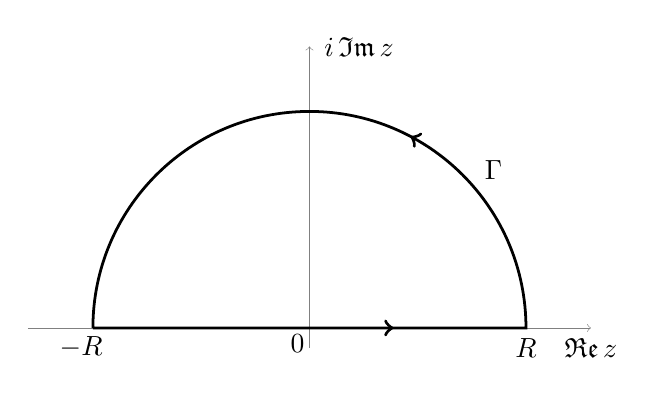
\begin{tikzpicture}
    \def\radius{2.75}

    \draw [help lines, ->] (-1.3 * \radius, 0) -- (1.3 * \radius, 0);

    \draw [help lines, ->] (0, -0.25) -- (0, 1.3 * \radius);

    \draw [line width=1pt, decoration={ markings, mark=at position
      0.27 with {\arrow[line width=1.2pt]{>}}, mark=at position 0.6
      with {\arrow[line width=1.2pt]{>}}}, postaction={decorate}]
    (-\radius, 0) -- (\radius, 0) arc (0:180:\radius);


    \node at (1.3 * \radius, -0.25) {$\mathfrak{Re}\, z$};

    \node at (0.63, 1.3 * \radius) {$i\, \mathfrak{Im}\, z$};


    \node at (-0.15, -0.2) {$0$};

    \node at (-\radius - 0.15, -0.25) {$-R$};

    \node at (\radius, -0.25) {$R$};

    \node at (0.85 * \radius, 2) {$\Gamma$};

  \end{tikzpicture}

  \caption{Jeden z~podstawowych konturów całkowania~$\Gamma$.}

  \label{fig:Leja-01}
\end{figure}
% ##################



\start \Str{32} Ze~względów praktycznych lepiej jest przyjąć,
że~kontur jest kawałkami gładką, a~nie po~prostu gładką, zorientowaną
dodatnio krzywą Jordana. W~praktyce bowiem do~najczęściej używanych
konturów są takie, które są tylko kawałkami gładkie, przykładem niech
będzie kontur~$\Gamma$ z~rysunku~(\ref{fig:Leja-01}).

W~tej chwili nie umiem rozstrzygnąć, czy~istnieje gładkie odwzorowanie
takie, że~jego obraz pokrywa~się z~kształtem~$\Gamma$ na~płaszczyźnie
zespolonej. Jednak nie jest to ważne, bowiem wykonując całkowanie
używa~się standardowo parametryzacji $\Gamma$, która gładka nie jest
(liniowej na~osi rzeczywistej, trygonometrycznej na~okręgu) i~nie
ma~żadnej praktycznej potrzeby by~taką była.

Należy zauważyć, że~pojęcie konturu używa~się w~praktyce nawet
w~ogólniejszych przypadkach, kiedy rozpatrywane krzywe mają punkty
wielokrotne. Takie jednak poszerzenie pojęcia konturu, odeszłoby
by~chyba zbyt daleko od~słów Lejii.

\vspace{\spaceFour}


\start \Str{33} Warto zaznaczyć, że~w~tej książce używa~się pojęcia
południk inaczej niż w~geografii, gdzie oznacza on~część okręgu
wielkiego biegnącą od~bieguna północnego do~południowego (półokrąg).
Tutaj natomiast oznacza okrąg wielki przechodzący przez oba bieguny
i~wydaje~się, że~terminologia ta jest używana w~całej książce
konsekwentnie.

\vspace{\spaceFour}


\start \Str{35} Warto byłoby udowodnić, że~jeśli punkty~$p$,~$q$ są
symetryczne względem pewnej prostej, to~łączący je odcinek jest
prostopadły do~tej prostej.

\vspace{\spaceFour}


\start \Str{36} Nazwanie prostych \textbf{okręgami niewłaściwymi}
i~\textbf{okręgami przechodzącymi przez punkt w nieskończoności} jest
to, że~rzucie stereograficznym obrazem okręgu na~sferze przechodzącego
przez biegun~$N$ jest właśnie linia prosta na~płaszczyźnie.

\vspace{\spaceFour}


\start \Str{38} Nie jestem pewien czy z~definicji wynika, że~do danych
pęków należą odpowiednie proste (okręgi niewłaściwe), czy też należy
tak zmodyfikować definicję, by~do nich należały.

\vspace{\spaceFour}


\start \Str{42} W~definicji ciała liczb wymiernych jest pewna
subtelność w~określeniu wyniku operacji dodawania, odejmowania,
mnożenia i~dzielenia. Rozważmy najpierw przypadek dzielenia. Wielomian
$P_{ 1 }( z ) = 1$ jest określony na~dziedzinie~$\C$. Jeśli podzielimy
go~przez wielomian $Q_{ 1 }( z ) = z - 1$ to otrzymany iloraz
$P_{ 1 }( z ) / Q_{ 1 }( z )$, to jest on określony na dziedzinie
$\C \setminus 1$, widzimy więc, że~operacja dzielenia może prowadzić
do~powstania funkcji o~nowej dziedzinie.

Teraz zajmiemy~się subtelniejszym problemem. Rozważmy następujący
iloczyn
\begin{equation}
  \label{eq:Leja-33}
  \begin{split}
    W_{ 1 }( z ) = \fr{ P_{ 1 }( z ) }{ Q_{ 1 }( z ) } ( z - 1 ) ( z -
    2 ) = \fr{ 1 }{ z - 1 } ( z - 1 ) ( z - 2 ) = z - 2.
  \end{split}
\end{equation}
Ponieważ funkcja $1 / ( z - 1 )$ jest określona tylko dla $z \neq 1$,
więc formalnie funkcja $W( z )$ ma~dziedzinę $\C \setminus 1$.
To~jedna mogłoby prowadzić do~niepotrzebnych komplikacji, na~przykład
okazałoby~się, że~$W( z ) \neq z - 2$ bo funkcje te mają różne
dziedziny. Z~tego problemu łatwo jednak wybrnąć.

Jeśli daną funkcję wymierną~$f( z )$ która jest określony na~zbiorze
$\C \setminus \set{ z_{ 1 }, z_{ 2 }, \ld, z_{ n } }$ można zapisać
w~postaci $P( z ) / Q( z )$ i~$z_{ i }$ nie jest zerem wielomianu $Q$,
wówczas zawsze rozszerzamy ją do~funkcji określonej na~zbiorze
$\C \setminus \set{ z_{ 1 }, z_{ 2 }, \ld, z_{ i - 1 }, z_{ i + 1 },
  \ld, z_{ n } }$ poprzez
\begin{equation}
  \label{eq:Leja-34}
  \begin{split}
    f( z_{ i } ) := \fr{ P( z_{ i } ) }{ Q( z_{ i } ) }.
  \end{split}
\end{equation}

\vspace{\spaceFour}


\start \Str{53} Warto byłoby tu częściej zaznaczać, że~liczba $N$ jest
funkcją argumentu zespolonego $N( z )$. Na~przykład pisząc
\begin{equation}
  \label{eq:Leja-35}
  \begin{split}
    f( z ) - \Sum_{ n = 0 }^{ N( z ) } a_{ n } \to 0.
  \end{split}
\end{equation}

\vspace{\spaceFour}


\start \Str{56} Definicja okresu funkcji zmiennej zespolonej jest
mniej jasna niż dla funkcji zmiennej rzeczywistej. Zwróćmy uwagę,
że~jeśli $w$ jest okresem funkcji to jest nim też~$2w$, ogólniej,
każda całkowita wielokrotność~$w$. Dla zmiennej rzeczywistej można
pojęcie okresu ujednoznacznić, wybierając najmniejszą liczbę dodatnią
o~podanych na~tej stronie własnościach. Jeśli~$w$ jest czysto
rzeczywista (lub~czysto urojona) jako okres należy przyjąć liczbę
której część rzeczywista (urojona) jest najmniejszą liczbą dodatnią
spośród możliwych. W~innym przypadku sformułowanie kryterium, który
z~okresów przyjąć, nie jest łatwe.

\vspace{\spaceFour}


\start \Str{56} Ze~wzoru (20) rzeczywiście wynika, że~$\sin$ i~$\cos$
mają okres $2\pi$, ale~nie wynika, iż~dla którejś z~nich nie~istnieje
mniejsza liczba dodatnia o~tej własności.

\vspace{\spaceFour}


\start \Str{58} Napotykamy tu ten sam problem, jaki omówiliśmy już
przy okazji $\arg z$. Wyrażenie $\log a$, przy ustalonym~$a$, nie
reprezentuje liczby zespolonej, lecz przeliczalny zbiór liczb. Dlatego
nieuważne stosowanie tej funkcji wielowartościowej, jakby była zwykła
funkcją, może prowadzić do~paradoksów, takich jakie powstają przy
stosowaniu wyrażenia~$\sqrt{ z }$. $\tr{Log}\, z$ jest już zwykłą
funkcją liczbową, choć nieciągłą, więc mając to w~pamięci można jej
używać w~zwykły sposób.

\vspace{\spaceFour}


\start \Str{59} Zamiast rozumieć przez $a^{ b }$ każdą z~liczb podanej
postaci, lepiej byłoby oznaczać zbiór wszystkich tych liczb.
Oczywiście, należy uważać na~wymienione już w~przypadku funkcji
wielowartościowych problemy.

\vspace{\spaceFour}


\start \Str{59--60} We~fragmencie o~gałęziach logarytmu należałoby
napisać, że~$l( z )$ ma być funkcją jednowartościową, inaczej
pojawia~się już problem na~poziomie tego co~ma znaczyć wyrażenie
$e^{ l( z ) }$. W~tym kontekście również argument z~nieciągłości
funkcji zdefiniowanej na~zbiorze zawierającym okrąg jest wątpliwy,
bo~powstaje problem, co oznacza ciągłość funkcji wielowartościowej?

Ostatecznie, zgodnie z~tym co zostało napisane o~$\arg z$, mamy dwa
wyjścia, jeśli chcemy określić gałąź logarytmu na~całej płaszczyźnie.
Albo~argumenty liczb zespolonych zmienia~się od~$-\infty$ do~$+\infty$
i~gałąź logarytmu przestaje być jednoznaczna, albo~ograniczamy ich
zakres na~przykład do~zbioru~$( -\pi, \pi ]$ i~wówczas funkcja musi
mieć skok, a~więc przestaje być ciągła.

\vspace{\spaceFour}


\start \Str{60} Nie udowodniono tu, że~dwie dowolne gałęzie logarytmu
różnią~się o~$2 k \pi i$. Dowód ten jest dość prosty.
\begin{equation}
  \label{eq:Leja-36}
  e^{ l_{ i }( z ) } = e^{ l_{ j }( z ) }
  \iff e^{ l_{ i }( z ) } / e^{ l_{ j }( z ) } = e^{ l_{ i }( z ) - l_{ j }( z ) }
  = 1.
\end{equation}
Wynika z~tego że~$l_{ i }( z ) - l_{ j }( z ) = 2 k( z ) \pi i$,
$k( z ) \in \Z$. Jako różnica dwóch funkcji ciągłych jest to~funkcja
ciągła, jednak funkcja ciągła o~wartościach całkowitych musi być równa
stałej, czyli $k( z ) = k \in \Z$.

\vspace{\spaceFour}


\start \Str{68} Należy przemyśleć, jaki jest sens tego, że~możemy
traktować $z$ i~$\zbar$ jako dwie zmienne niezależne.

\vspace{\spaceFour}


\start \Str{68} W~podany tu~twierdzeniu o~związku między pochodną
zespoloną, a~formalną kluczowe jest to, że~zakłada~się w~nim, iż
pochodne cząstkowe istnieją i~są ciągłe. Założenie to zostało podane
wyżej w~tekście, niestety nie zostało przedstawione jawnie w~treści
twierdzenia.

\vspace{\spaceFour}


\start \Str{73} Przedyskutujemy tu~czy rysunek~(36) poprawnie
przedstawia działanie funkcji analitycznej w~otoczeniu punktu
$z_{ 0 }$ takiego, że~$f'( z_{ 0 } ) \neq 0$. Okazuje~się, że~w~pewnym
otoczeniu tego punktu funkcja istotnie musi zachowywać~się tak, jak to
tam przedstawiono. Aby~ninijesza analiza była prawomocna należy
założyć, że~funkcje $u( x, y )$, $v( x, y )$ są odpowiednio gładkie.
Choć potem zostanie pokazane, że~są one klasy
$\Cinfty( \Rtwo )$\footnote{Dokładniej: są one analityczne na~$\Rtwo$.
  Jednak do~tej pory nie znalazłem dowodu tego faktu w~książce
  Lejii.}, to tutaj wystarczy nam, że~są klasy
$\Cone( \Rtwo )$\footnote{Należy sprawdzić, czy nie wystarczy zwykła
  różniczkowalność.}.

Zacznijmy od~uwagi ogólnej. Jeśli oznaczymy
$z_{ 0 } = x_{ 0 } + i y_{ 0 }$, $c = u( x_{ 0 }, y_{ 0 } )$
i~$c' = v( x_{ 0 }, y_{ 0 } )$, to~równania $c = u( x, y )$
i~$c' = v( x, y )$ wyznaczają poziomice funkcji $u( x, y )$
do~wartości~$c$ i~$v( x, y )$ do~wartości~$c'$. Ze~wzoru (18)
na~stronie~72 wiemy, że~jeśli $f'( z_{ 0 } ) \neq 0$, to macierz
Jacobiego odwzorowania $( u( x, y ), v( x, y ) )$ jest w tym punkcie
nieosobliwa. Na~mocy twierdzenia o~lokalnym odwracaniu odwzorowań
istnieje otoczenie punktu $z_{ 0 } \in \mathcal{V}$ takie, że~na
$f( \mathcal{V} )$ istnieje odwzorowanie $f^{ -1 }$, które jest tak
gładkie jak funkcje $u( x, y )$ i~$v( x, y )$. Na~podstawie tego oraz
równań Cauchy'ego-Riemanna można pokazać, że~na zbiorze $\mathcal{V}$
sytuacja musi wyglądać tak, jak na rysunku~(36).

Jako, że~nie musi to być całkiem oczywiste tutaj przedstawimy dyskusję
kilku wynikających stąd własności. Kąt pod jakim przecinają~się
poziomice, jak pokazano w~książce, wynika z~równań
Cauchy'ego-Riemanna. Poziomica $c = u( x, y )$ (analogicznie
rozumujemy dla $c' = v( x, y )$) jest obrazem przez funkcję $f^{ -1 }$
przecięcia prostej $u = c$ i~zbioru $f( \mathcal{V} )$, na~mocy więc
bijektywności~$f^{ -1 }$ pokrywają one cały zbiór $\mathcal{V}$. Ich
gładkość zaś~wynika z~gładkości~$f^{ -1 }$. Co więcej, ponieważ
w~zbiorze $f( \mathcal{V} )$ proste $c = u$ i~$c' = v$ przecinają~się
tylko raz, więc na~mocy injektywności $f$, również odpowiadające
im~poziomice przecinają~się tylko raz w~zbiorze~$\mathcal{V}$.

Nie ma potrzeby zajmować~się globalnym kształtem poziomic, więc
zagadnienia tego nie będziemy omawiać.

\vspace{\spaceFour}


\start \Str{74} Osie $\eta$ i~$\xi$ na~rys.~38~są podpisane na~odwrót.

\vspace{\spaceFour}


\start \Str{75} Wskazówka do~obliczenia wzorów (23): na~początku
policz~$\abso{ z }^{ 2 } + 1$.

\vspace{\spaceFour}


\start \Str{75} W~opisie rzutu Merkatora zabrakło wyjaśnienia,
po~której stronie równika należy umieścić rzut punktu~$z'$. Wynika
to~jednak jasno z~rysunku.

\vspace{\spaceFour}


\start \Str{75} Stwierdzenie, że~pochodna homografii jest wszędzie
różna od~0, jest problematyczne, bowiem nie jest wcale jasne,
czy~można przypisać jakiś sens pochodnej w~punkcie $z = -d / c$.
Prawdą jest jednak, że~pochodna homografii jest różna od~0 wszędzie
poza tym punktem.

\vspace{\spaceFour}


\start \Str{79} Ponieważ jak to zostało wspomniane w~komentarzu
do~str.~10, $\arg z$ jest funkcją wieloznaczną, co~rodzi pewne
nieoczekiwane trudności przy posługiwaniu~się nią, więc zapewne też
funkcja $\vp( x, y ) = \arg f( z )$, będzie sprawiać podobne
trudności. Z~tego powodu również poziomica $\mu' = \vp( x, y )$ może
być znacznie bardziej skomplikowany obiektem, niż byśmy oczekiwali.

Jednak lokalnie zarówno postać biegunowa, jak i~odpowiadające jej
poziomice powinny być dobrze określone. Może warto będzie do~tego
zagadnienia powrócić i~zanalizować je dokładnie?

\vspace{\spaceFour}


\start \Str{87--88} Udowodniono to, że~$I( C, a )$ jest liczbą
całkowitą, jednak warto byłoby podać jakieś argumenty za~tym,
że~rzeczywiście równa jest ona liczbie obiegów, liczonych ze~zwrotem,
wokół punktu~$a$ krzywej zamkniętej~$C$.

Należy też dodać komentarz, że~okrążenie punktu przez krzywą liczymy
ze~znakiem plus, gdy~podczas okrążania krzywa jest zorientowana
dodatnio względem swojego wnętrza, ze~znakiem minus, gdy~jest
zorientowana ujemnie. To~rodzi problem jak zdefiniować wnętrze krzywej
zamkniętej z~samoprzecięciami, odłóżmy go~jednak na~inny czas.

\vspace{\spaceFour}


\start \Str{92} W~tym miejscu chyba wychodzi założenie, że~pracujemy
tylko z~krzywymi przedziałami gładkimi. W~przeciwnym bowiem razie
krzywa ta~mogłaby nie mieć określonej długości albo~mogłoby nie
dać~się aproksymować ją przez linię łamaną.

\vspace{\spaceFour}


\start \Str{93} Sytuacja przedstawiona na~rysunku~52 wymaga
zadziwiająco dużo twierdzeń z~topologii płaszczyzny i~krzywych,
których dowody wcale nie~są dla mnie oczywiste. Po pierwsze,
że~istnieją łuki regularne~$l_{ i }$ łączące kontur~$C_{ 0 }$
z~konturami $C_{ i }$ i~że~powstała w~wyniku tej konstrukcji krzywa
jest wciąż kawałkami gładka. Po~drugie należy udowodnić, że~w~tej
nowej krzywej znajdują~się wszystkie krzywe $-C_{ i }$ i~po każdej
z~nich całkujemy dokładnie raz, brak zaś w~ogóle $C_{ i }$.
Po~trzecie, że~po~każdym z~łuków $l_{ i }$ całkujemy dokładnie dwa
razy, obiegając je w~dwóch przeciwnych kierunkach.

Wszystkie te~stwierdzenia~są oczywiste na~podstawie rysunku, więc jest
zrozumiałe, że~Leja chciał uniknąć dowodzenia ich wszystkich.

\vspace{\spaceFour}


\start \Str{94} Wprowadzono tu~pojęcie sumy krzywych, jednak nie
zostało one w~żaden sposób jasno zdefiniowane, pozostając na~poziomie
intuicji matematycznej.

\vspace{\spaceFour}


\start \Str{94} W~tym miejscu chyba pierwszy raz pojawia~się pojęcie
,,drogi całkowania'', jednak nie jest ono zdefiniowane. Przez
\textbf{drogę całkowania} należy rozumieć krzywą kawałkami gładką. Dla
wygody będziemy czasem mówili po~prostu o~,,drodze''.

\vspace{\spaceFour}



% ##################
\begin{figure}
  \centering

  \begin{tikzpicture}[scale=1.35]
    \def\scale{2.5} \def\R{2.6}

    \draw [help lines, ->] (0, 0) -- (\scale, 0);

    \draw [help lines, ->] (0, -0.5) -- (0, \scale);

    \draw [dashed] (-0.6 * \scale, 0) -- (0, 0);

    \draw [line width=0.9pt, decoration={ markings, mark=at position
      0.2 with {\arrow[line width=1.2pt]{>}}, mark=at position 0.6
      with {\arrow[line width=1.1pt]{>}}}, postaction={decorate}] (1,
    0) arc (0:55:1) -- (0.57 * \R, 0.82 * \R);

    % Kod w elispie do obliczania funkcji trygonometrycznych
    % (cos (* pi (/ 55.0 180)))
    % (sin (* pi (/ 55.0 180)))


    \filldraw [black] (1, 0) circle (1.5pt) node [anchor=north] {1};

    \filldraw [black] (0.57, 0.82) circle (1pt) node [anchor=east]
    {$e^{ i \varphi }$};

    \filldraw [black] (0.57 * \R, 0.82 * \R) circle (1.5pt) node
    [anchor=west] {$R\, e^{ i \varphi }$};

    \node at (1.0, 0.65) {$\Gamma$};


    \node at (0.5, \scale) {$i\, \mathfrak{Im}\, z$};

    \node at (\scale, -0.25) {$\mathfrak{Re}\, z$};

  \end{tikzpicture}

  \caption{Przykładowy kontur po~którym można całkować funkcje
    $1 / \zeta$ ,,od~1 do~nieskończoności''.}

  \label{fig:Leja-02}
\end{figure}
% ##################



\start \Str{95} W~twierdzeniu o~istnieniu jednoznacznej gałęzi
logarytmu zakładamy, że~dany obszar~$D$ jest jednospójny i~nie zawiera
$0$ i~$\infty$. Dlaczego musi byś jednospójny jest oczywiste,
kontrprzykład z~okręgiem ze~stron~59--60 pokazuje, gdzie leży problem.
Wykluczenie~$0$ też jest jasne, mówienie o~analityczności $1 / \zeta$
w~zerze nie ma sensu. Większe problemy stwarza potrzeba usunięcia
punktu~$\infty$.

Istnieją po~temu dwa powody. Po pierwsze, zgodnie z~przyjęto
definicjom jednospójności zbiór
$\C \cap \set{ \infty } \setminus \set{ 0 }$ byłby jednospójny,
a~twierdzenie dla niego jawnie nie zachodzi. Jeśli z~rozważanego
zbioru wykluczymy $0$ i~$\infty$ to, aby był jednospójny musimy
z~niego wykluczyć też odpowiedni zbiór ,,łączący'' te~dwa punkty,
np.~prostą $\Real\, z < 0$, wykluczający tym samym z~rozważań
wszystkie nieporządne zbiory.

Drugi powód jest następujący. Rozpatrzmy jak na
rysunku~(\ref{fig:Leja-02}) płaszczyznę zespoloną bez osi
$\Real\, z \leq 0$. Można sobie zadać pytanie, czy~wartość całki
z~$1 / \zeta$ po~konturze $\gamma_{ R }$ jest zbieżna, gdy kontur
całkowania $\gamma_{ R }$ o~początku $a$ rozciągamy
,,do~nieskończoności'' (dla prostoty przyjmijmy $a = 1$). Przez to
ostatnie stwierdzenie rozumiemy, że~rozważamy rodzinę konturów
$\gamma_{ R }: [ t_{ 0 }, t_{ 1 } ] \to \C$ takich, że
\begin{equation}
  \label{eq:Leja-38}
  \Lim_{ \RToInf } \gamma_{ R }( t_{ 1 } ) = \infty.
\end{equation}
Ponieważ wartość z~całki $1 / \zeta$ nie zależy od~drogi wystarczy
posłużyć~się rodziną konturów $\gamma_{ R }$ przedstawioną na
rysunku~(\ref{eq:Leja-02}). Nietrudne obliczenia pokazują, że~całka
ta~jest zbieżna przy~$\RToInf$, do~$\infty$, niezależnie
od~wartości~$\varphi$.

Jakkolwiek można by więc nadać sens logarytmowi od~$\infty$, to~byłby
wówczas pewien problem z~zależnością $\exp( \log z ) = z$. Nie
istnieje bowiem żaden naturalny wybór wartości $\exp( \infty )$,
bowiem
\begin{equation}
  \label{eq:Leja-39}
  \begin{split}
    \Lim_{ \xToPInf } e^{ x } = +\infty, \quad \Lim_{ \xToMInf } e^{
      -x } = 0, \quad x \in \R.
  \end{split}
\end{equation}
Trzeba by więc przyjąć, że~$\exp( \infty ) = \infty$, by~zachodził
wzór $\exp( \log \infty ) = \infty$. Biorąc to~wszystko pod uwagę,
decyzja by wykluczyć z~rozważanego zbioru $D$ punkt $\infty$, jawi~się
jako dobrze uzasadniona.

\vspace{\spaceFour}


\start \Str{96} Dowód, że~w~obszarze jednospójnym funkcja
$\log f( z )$ istnieje jest w~tym momencie niepełny. Ponieważ
założyliśmy, że~funkcji $f( z )$ jest analityczna, w~tym momencie
wiemy tylko, że~istnieje jej pierwsza pochodna. Z~tego względu nie
możemy twierdzić, że~$f'( z ) / f( z )$ jest różniczkowalna, tym samym
analityczna. Dopiero gdy dowiedziemy, że~każda funkcja analityczna
jest nieskończenie wiele razy różniczkowalna, dowód będzie pełen.

\vspace{\spaceFour}


\start \Str{102} Pokazano tu, że~jeśli funkcja analityczna ma~0
skończonego rzędu, to~pewnym jego otoczeniu nie przyjmuje wartości~0.
Z~tego chyba jednak nie wynika od~razu, że~jeśli zeruje~się na~zbiorze
posiadającym punkt skupienia wewnątrz obszaru określoności~$D$,
to~zeruje~się w~całym~$D$.

Aby to udowodnić potrzebne nam będzie następujący lemat. Jeśli funkcja
analitycznej $f( z )$ określona w~obszarze~$D$, jest równa zeru
w~pewnym zbiorze otwartym to~zbiór ten jest równy $\emptyset$
albo~$D$. Rozpatrzmy zbiór $E$ takich punktów, że~$f( z )$ jest równa
zeru w~otoczeniu każdego z~nich. Jest to zbiór otwarty, gdyż
\begin{equation}
  \label{eq:Leja-40}
  E = \bigcup_{ z \in E } \Oc_{ z },
\end{equation}
gdzie $\Oc_{ z }$ jest takim otoczeniem punktu $z$, że~$f( z )$ znika
w~nim. Niech teraz $w_{ 0 } \in D$ będzie punktem skupienia zbioru $E$
i~niech $w_{ n } \in E$ będzie ciągiem elementów zbieżnym
do~$w_{ 0 }$. Funkcja $f( z )$ jest ciągła w~$D$, bo~posiada pochodną
$f'( z )$, stąd
\begin{equation}
  \label{eq:Leja-41}
  f( w_{ 0 } ) = \Lim_{ \nToInfty } f( w_{ n } ) = 0.
\end{equation}
Analogicznie $f'( z )$ jest ciągła na mocy istnienia~$f''( z )$
i~powtarzając powyższe rozumowanie otrzymujemy,
że~$f'( w_{ 0 } ) = 0$. Kontynuując to~rozumowanie pokazujemy,
że~$f^{ ( k ) }( w_{ 0 } ) = 0$, $k = 0, 1, 2, \ldots$ Ponieważ
znikają wszystkie wyrazy rozwinięcia $f( z )$ w~szereg Taylora
w~punkcie $w_{ 0 }$ i~szereg ten musi mieć niezerowy promień
zbieżności, funkcja~$f( z )$ znika pewnym otoczeniu~$w_{ 0 }$ i~tym
samym $w \in E$.

Ponieważ $E$ jest jednocześnie otwarty i~domknięty w~$D$, a~$D$ jako
obszar jest zbiorem spójnym, $E = \emptyset$ lub $E = D$.

Przejdźmy do~dowodu zasadniczego twierdzenia. Jeśli funkcja $f( z )$
zeruje~się na zbiorze posiadającym punkt skupienia $z_{ 0 } \in D$, to
w~$z_{ 0 }$ muszą znikać wszystkie wyrazy jej szeregu Taylora, na~mocy
tego co pokazał Leja. Ponownie korzystając z~tego, że~promień
zbieżności tego szeregu jest niezerowy, widzimy, że~funkcja~$f( z )$
znika w~kole otwartym o~niezerowym promieniu, więc na~mocy
poprzedniego lematu znika w~całym~$D$.

\vspace{\spaceFour}


\start \textbf{Str.~106, wiersze 1--2.} Nierówność
$\abso{ f( z' ) } > \abso{ f( z_{ 0 } ) }$ jest bardzo brzydko
podzielona między dwie linie.

\vspace{\spaceFour}


\start \Str{132} Podobnie jak przy definiowaniu ciała funkcji
wymiernych, należy tu~dodać komentarz, że~jeśli funkcja $f( z )$ ma
w~punkcie $z_{ 0 }$ biegun, to~definiujemy $1 / f( z_{ 0 } ) := 0$.

\vspace{\spaceFour}


\CenterTB{Błędy}
\begin{center}
  \begin{tabular}{|c|c|c|c|c|}
    \hline
    & \multicolumn{2}{c|}{} & & \\
    Strona & \multicolumn{2}{c|}{Wiersz} & Jest
                              & Powinno być \\ \cline{2-3}
    & Od góry & Od dołu & & \\
    \hline
    7   & & 10 & $\al,\:\; \be$ & $\al, \be$ \\
    7   & &  9 & $x,\! y$ & $x, y$ \\
    11  &  2 & & $\abso{ a b }$ & $ab$ \\
    11  &  3 & & $\abso{ \tfr{ a }{ b } }$ & $\tfr{ a }{ b }$ \\
    22  &  1 & & $\al_{ n }$ & $\al_{ n - 1 }$ \\
    22  &  1 & & $\be_{ n }$ & $\be_{ n - 1 }$ \\
    22  & 13 & & urojoną ? & urojoną? \\
    22  & 15 & & rzeczywistą~? & rzeczywistą? \\
    24  & 11 & & $a, \:\; b$ & $a, b$ \\
    25  & &  6 & $\tr{re}\, z < 0$ & $\tr{re}\, z = 0$ \\
    27  & &  9 & wniosek~: & wniosek: \\
    27  &  6 & & zbieżny, & zbieżny. \\
    27  & &  2 & Spójność & $N$-spójność \\
    29  &  6 & & otwarty~: & otwarty: \\
    30  & & 13 & $t$ & $( t - t_{ 0 } )$ \\
    30  & & 11 & $t$ & $( t - t_{ 0 } )$ \\
    36  &  2 & & $\tr{re}( \ol{ p } - \la^{ 2 } \ol{ q } ) z$
           & $\tr{re}[( \ol{ p } - \la^{ 2 } \ol{ q } ) z]$ \\
    36  &  4 & & $\left| \frac{ z - ( p - \uplambda^{ 2 } q) }{ 1
                 - \uplambda^{ 2 } } \right|^{ 2 }$
           & $\left| z - \frac{ ( p - \uplambda^{ 2 } q) }{ 1
             - \uplambda^{ 2 } } \right|^{ 2 }$ \\
    39  &  2 & & $\abso{ b - c }$ ? & $\abso{ b - c }$? \\
    45  & 13 & & \emph{wewnętrzną ,} & \emph{wewnętrzną,} \\
    47  &  5 & & $z_{ n }$ & $z^{ n }$ \\
    49  & & 13 & $\sqrt[n]{ \abso{ a_{ n } } } z$
           & $\sqrt[n]{ \abso{ a_{ n } } } | z |$ \\
    53  &  7 & & $s$ ? & $s$? \\
    54  & 10 & & słabszym : & słabszym: \\
    56  & &  4 & w~zbiorze & \emph{w~zbiorze} \\
    57  &  9 & & 31 & 31) \\
    64  &  5 & & krótko : & krótko: \\
    65  & & 14 & \emph{jeśli ma} & \emph{ma} \\
    68  & 16 & & $\pd{}{ f }{ z } - i \pd{}{ f }{ y }$
           & $\pd{}{ f }{ x } - i \pd{}{ f }{ y }$ \\
    69  & & 13 & $a_{ n }$ & $\abso{ a_{ n } }$ \\
    73  & 13 & & $iw$ & $iv$ \\
    75  & &  7 & $( a z_{ 1 } + b )\;\, ( c z_{ 2 } + d )$
           & $( a z_{ 1 } + b ) ( c z_{ 2 } + d )$ \\
    75  & &  3 & $c z - d$ & $c z + d$ \\
    75  & & 16 & $ab - bc$ & $ad - bc$ \\
    79  & &  5 & okręgów~: & okręgów: \\
    80  & & 12 & $a^{ x } \cdot a^{ iy }$ & $e^{ x } \cdot e^{ iy }$ \\
    80  & & 10 & prostą~: & prostą: \\
    90  &  2 & & \emph{krzywą zamkniętą} & \emph{konturem} \\
    \hline
  \end{tabular}

  \begin{tabular}{|c|c|c|c|c|}
    \hline
    & \multicolumn{2}{c|}{} & & \\
    Strona & \multicolumn{2}{c|}{Wiersz} & Jest
                              & Powinno być \\ \cline{2-3}
    & Od góry & Od dołu & & \\
    \hline
    90  &  5 & & pochodna$f'( z )$ & pochodna $f'( z )$ \\
    92  & &  6 & \emph{krzywą} & \emph{krzywą kawałkami gładką} \\
    94  & &  6 & regularną & kawałkami gładką \\
    99  &  1 & & zewnątrz & na~zewnątrz \\
    102 & 14 & & $=\!\! f^{ ( k - 1 ) }( z_{ 0 } )$
           & $= f^{ ( k - 1 ) }( z_{ 0 } )$ \\
    102 & &  7 & części & części otwartej \\
    105 & &  6 & zerowych : & zerowych: \\
    106 & &  2 & \emph{jest w~środku} & \emph{w~środku} \\
    106 & &  1 & \emph{równa} & \emph{jest równa} \\
    107 &  6 & & $\abso{ z } \leq r$ & $\abso{ z } = r$ \\
    119 & 15 & & $K \{ \abso{ z - z_{ 0 } } < R \}$
           & $K = \{ \abso{ z - z_{ 0 } } < R \}$ \\
    131 & 11 & & myś & myśl \\
    126 & &  7 & $\frac{ ( \zeta - z_{ 0 } )^{ n } }{
                 ( z - z_{ 0 } )^{ n + 1 } }$
           & $\frac{ ( z - z_{ 0 } )^{ n } }{
             ( \zeta - z_{ 0 } )^{ n + 1 } }$ \\
    132 &  2 & & $=\!\! a_{ -k + 1 }$ & $= a_{ -k + 1 }$ \\
    134 & 14 & & $P_{ 3 }( a )$ & $P_{ 3 }( z )$ \\
    140 & &  7 & $f |$ & $\abso{ f }$ \\
    143 & & 18 & w~otoczeniu punktu & \emph{w~otoczeniu punktu} \\
    166 &  6 & & potęgowych . & potęgowych. \\
    199 &  3 & & $\nu = 1 $ & $k = 1$ \\
    % & & & & \\
    % & & & & \\
    % & & & & \\
    % & & & & \\
    % & & & & \\
    % & & & & \\
    % & & & & \\
    % & & & & \\
    % & & & & \\
    \hline
  \end{tabular}
\end{center}
\noi \\
\StrWg{28}{5} \\
\Jest nieograniczone \\
\Pow  nieograniczone i~domknięte \\
\StrWg{36}{5} \\
\Jest Ze~wzorów (9)~otrzymujemy \\
\Pow  Otrzymujemy z~nich wzory~(9) i~na ich mocy mamy \\
\StrWg{56}{2} \\
\Jest a~istnieją wartości~$w$, które \\
\Pow  a~istnieje wartość~$w$, którą \\
\StrWg{75}{12} \\
\Jest rozciętej wzdłuż jednego południka na~pas nieograniczony
płaszczyzny~$p$ nawiniętej na~powierzchnię boczną \\
\Pow rzutowanej wzdłuż południków na~pas nieograniczony~$p$ zwinięty
w~powierzchnię boczną \\
\StrWg{95}{5} \\
\Jest linią \\
\Pow dowolna linia łamana \\
\StrWd{107}{12} \\
\Jest dowolnym konturem zawartym \\
\Pow  dowolną drogą całkowania zawartą \\
\StrWd{108}{13} \\
\Jest domkniętym \\
\Pow  domkniętym i~ograniczonym \\
\StrWd{119}{8} \\
\Jest \emph{są~identyczne, jeżeli~są równe na~brzegu~$B$} \\
\Pow \emph{jeśli~są równe na~brzegu $B$, to~są równe również
  w~obszarze~$D$} \\
\StrWd{134}{16} \\
\Jest krzywych zamkniętych \\
\Pow  kawałkami gładkich zamkniętych krzywych \\

\vspace{\spaceTwo}





% % ####################
% \Work{ % Autor i tytuł dzieła
% B. W. Szabat \\
% ,,Wstęp do analizy zespolonej'',
% \cite{SzabatWstepDoAnalizyZespolonej1974} }


% \CenterTB{Błędy}
% \begin{center}
%   \begin{tabular}{|c|c|c|c|c|}
%     \hline
%     & \multicolumn{2}{c|}{} & & \\
%     Strona & \multicolumn{2}{c|}{Wiersz} & Jest
%                               & Powinno być \\ \cline{2-3}
%     & Od góry & Od dołu & & \\
%     \hline
%     17  &  5 & & dal & dal\dywiz \\
%     25  & & 11 & $z_{ 2 }( t )$ & $z_{ 2 }( \tau( t ) )$ \\
%     %     & & & & \\
%     \hline
%   \end{tabular}
% \end{center}

% \vspace{\spaceTwo}






% ####################################################################
% ####################################################################
% Bibliografia
\bibliographystyle{plalpha} \bibliography{LibMathInfo}{}



% ############################

% Koniec dokumentu
\end{document}
